\documentclass[twoside]{book}

% Packages required by doxygen
\usepackage{fixltx2e}
\usepackage{calc}
\usepackage{doxygen}
\usepackage[export]{adjustbox} % also loads graphicx
\usepackage{graphicx}
\usepackage[utf8]{inputenc}
\usepackage{makeidx}
\usepackage{multicol}
\usepackage{multirow}
\PassOptionsToPackage{warn}{textcomp}
\usepackage{textcomp}
\usepackage[nointegrals]{wasysym}
\usepackage[table]{xcolor}

% Font selection
\usepackage[T1]{fontenc}
\usepackage[scaled=.90]{helvet}
\usepackage{courier}
\usepackage{amssymb}
\usepackage{sectsty}
\renewcommand{\familydefault}{\sfdefault}
\allsectionsfont{%
  \fontseries{bc}\selectfont%
  \color{darkgray}%
}
\renewcommand{\DoxyLabelFont}{%
  \fontseries{bc}\selectfont%
  \color{darkgray}%
}
\newcommand{\+}{\discretionary{\mbox{\scriptsize$\hookleftarrow$}}{}{}}

% Page & text layout
\usepackage{geometry}
\geometry{%
  a4paper,%
  top=2.5cm,%
  bottom=2.5cm,%
  left=2.5cm,%
  right=2.5cm%
}
\tolerance=750
\hfuzz=15pt
\hbadness=750
\setlength{\emergencystretch}{15pt}
\setlength{\parindent}{0cm}
\setlength{\parskip}{3ex plus 2ex minus 2ex}
\makeatletter
\renewcommand{\paragraph}{%
  \@startsection{paragraph}{4}{0ex}{-1.0ex}{1.0ex}{%
    \normalfont\normalsize\bfseries\SS@parafont%
  }%
}
\renewcommand{\subparagraph}{%
  \@startsection{subparagraph}{5}{0ex}{-1.0ex}{1.0ex}{%
    \normalfont\normalsize\bfseries\SS@subparafont%
  }%
}
\makeatother

% Headers & footers
\usepackage{fancyhdr}
\pagestyle{fancyplain}
\fancyhead[LE]{\fancyplain{}{\bfseries\thepage}}
\fancyhead[CE]{\fancyplain{}{}}
\fancyhead[RE]{\fancyplain{}{\bfseries\leftmark}}
\fancyhead[LO]{\fancyplain{}{\bfseries\rightmark}}
\fancyhead[CO]{\fancyplain{}{}}
\fancyhead[RO]{\fancyplain{}{\bfseries\thepage}}
\fancyfoot[LE]{\fancyplain{}{}}
\fancyfoot[CE]{\fancyplain{}{}}
\fancyfoot[RE]{\fancyplain{}{\bfseries\scriptsize Generated by Doxygen }}
\fancyfoot[LO]{\fancyplain{}{\bfseries\scriptsize Generated by Doxygen }}
\fancyfoot[CO]{\fancyplain{}{}}
\fancyfoot[RO]{\fancyplain{}{}}
\renewcommand{\footrulewidth}{0.4pt}
\renewcommand{\chaptermark}[1]{%
  \markboth{#1}{}%
}
\renewcommand{\sectionmark}[1]{%
  \markright{\thesection\ #1}%
}

% Indices & bibliography
\usepackage{natbib}
\usepackage[titles]{tocloft}
\setcounter{tocdepth}{3}
\setcounter{secnumdepth}{5}
\makeindex

% Hyperlinks (required, but should be loaded last)
\usepackage{ifpdf}
\ifpdf
  \usepackage[pdftex,pagebackref=true]{hyperref}
\else
  \usepackage[ps2pdf,pagebackref=true]{hyperref}
\fi
\hypersetup{%
  colorlinks=true,%
  linkcolor=blue,%
  citecolor=blue,%
  unicode%
}

% Custom commands
\newcommand{\clearemptydoublepage}{%
  \newpage{\pagestyle{empty}\cleardoublepage}%
}

\usepackage{caption}
\captionsetup{labelsep=space,justification=centering,font={bf},singlelinecheck=off,skip=4pt,position=top}

%===== C O N T E N T S =====

\begin{document}

% Titlepage & ToC
\hypersetup{pageanchor=false,
             bookmarksnumbered=true,
             pdfencoding=unicode
            }
\pagenumbering{alph}
\begin{titlepage}
\vspace*{7cm}
\begin{center}%
{\Large Vector \\[1ex]\large 1.\+0 }\\
\vspace*{1cm}
{\large Generated by Doxygen 1.8.13}\\
\end{center}
\end{titlepage}
\clearemptydoublepage
\pagenumbering{roman}
\tableofcontents
\clearemptydoublepage
\pagenumbering{arabic}
\hypersetup{pageanchor=true}

%--- Begin generated contents ---
\chapter{Data Structure Index}
\section{Data Structures}
Here are the data structures with brief descriptions\+:\begin{DoxyCompactList}
\item\contentsline{section}{\hyperlink{classVector_3_01bool_01_4_1_1BoolReference}{Vector$<$ bool $>$\+::\+Bool\+Reference} }{\pageref{classVector_3_01bool_01_4_1_1BoolReference}}{}
\item\contentsline{section}{\hyperlink{classVector}{Vector$<$ data $>$} \\*Type \hyperlink{classVector}{Vector}. Effective in speed, but spends a lot of memory }{\pageref{classVector}}{}
\item\contentsline{section}{\hyperlink{classVector_3_01bool_01_4}{Vector$<$ bool $>$} \\*Type \hyperlink{classVector_3_01bool_01_4}{Vector$<$bool$>$}. Effective in speed, but spends a lot of memory }{\pageref{classVector_3_01bool_01_4}}{}
\end{DoxyCompactList}

\chapter{File Index}
\section{File List}
Here is a list of all documented files with brief descriptions\+:\begin{DoxyCompactList}
\item\contentsline{section}{\hyperlink{den__exception_8cpp}{den\+\_\+exception.\+cpp} \\*Special exception class }{\pageref{den__exception_8cpp}}{}
\item\contentsline{section}{\hyperlink{main_8cpp}{main.\+cpp} \\*Some example of \hyperlink{classDenException}{Den\+Exception} }{\pageref{main_8cpp}}{}
\end{DoxyCompactList}

\chapter{Data Structure Documentation}
\hypertarget{classVector_3_01bool_01_4_1_1BoolReference}{}\section{Vector$<$ bool $>$\+:\+:Bool\+Reference Class Reference}
\label{classVector_3_01bool_01_4_1_1BoolReference}\index{Vector$<$ bool $>$\+::\+Bool\+Reference@{Vector$<$ bool $>$\+::\+Bool\+Reference}}
\subsection*{Public Member Functions}
\begin{DoxyCompactItemize}
\item 
\hyperlink{classVector_3_01bool_01_4_1_1BoolReference_a7b319cb4b874379cbeb6d303b5d323eb}{Bool\+Reference} (int $\ast$bool\+\_\+pointer, int position)
\begin{DoxyCompactList}\small\item\em constructor  create a \hyperlink{classVector_3_01bool_01_4_1_1BoolReference}{Bool\+Reference} \end{DoxyCompactList}\item 
\mbox{\Hypertarget{classVector_3_01bool_01_4_1_1BoolReference_a9a6a68833363cc0ed810862d38f22f0a}\label{classVector_3_01bool_01_4_1_1BoolReference_a9a6a68833363cc0ed810862d38f22f0a}} 
\hyperlink{classVector_3_01bool_01_4_1_1BoolReference_a9a6a68833363cc0ed810862d38f22f0a}{$\sim$\+Bool\+Reference} ()
\begin{DoxyCompactList}\small\item\em destructor  free \hyperlink{classVector_3_01bool_01_4_1_1BoolReference}{Bool\+Reference} \end{DoxyCompactList}\item 
\hyperlink{classVector_3_01bool_01_4_1_1BoolReference_a7b319cb4b874379cbeb6d303b5d323eb}{Bool\+Reference} \& \hyperlink{classVector_3_01bool_01_4_1_1BoolReference_a5d76de9a5ad35583fe447af9951d1491}{operator=} (const bool value)
\begin{DoxyCompactList}\small\item\em operator= \end{DoxyCompactList}\item 
\hyperlink{classVector_3_01bool_01_4_1_1BoolReference_a56531a72bf638739e704e8fb07b0f394}{operator bool} () const
\begin{DoxyCompactList}\small\item\em operator bool() \end{DoxyCompactList}\end{DoxyCompactItemize}
\subsection*{Private Attributes}
\begin{DoxyCompactItemize}
\item 
\mbox{\Hypertarget{classVector_3_01bool_01_4_1_1BoolReference_ad9fc66c2a80d7351e5829e321c4d46f0}\label{classVector_3_01bool_01_4_1_1BoolReference_ad9fc66c2a80d7351e5829e321c4d46f0}} 
int $\ast$ \hyperlink{classVector_3_01bool_01_4_1_1BoolReference_ad9fc66c2a80d7351e5829e321c4d46f0}{bool\+\_\+pointer\+\_\+}
\begin{DoxyCompactList}\small\item\em pointer to int cell \end{DoxyCompactList}\item 
\mbox{\Hypertarget{classVector_3_01bool_01_4_1_1BoolReference_a88f229e6c448c4e7f34381247eb7f2b8}\label{classVector_3_01bool_01_4_1_1BoolReference_a88f229e6c448c4e7f34381247eb7f2b8}} 
int \hyperlink{classVector_3_01bool_01_4_1_1BoolReference_a88f229e6c448c4e7f34381247eb7f2b8}{position\+\_\+}
\begin{DoxyCompactList}\small\item\em position in int cell \end{DoxyCompactList}\end{DoxyCompactItemize}


\subsection{Detailed Description}
\subsubsection*{template$<$$>$\newline
class Vector$<$ bool $>$\+::\+Bool\+Reference}



Definition at line 32 of file bool\+\_\+vector.\+cpp.



\subsection{Constructor \& Destructor Documentation}
\mbox{\Hypertarget{classVector_3_01bool_01_4_1_1BoolReference_a7b319cb4b874379cbeb6d303b5d323eb}\label{classVector_3_01bool_01_4_1_1BoolReference_a7b319cb4b874379cbeb6d303b5d323eb}} 
\index{Vector$<$ bool $>$\+::\+Bool\+Reference@{Vector$<$ bool $>$\+::\+Bool\+Reference}!Bool\+Reference@{Bool\+Reference}}
\index{Bool\+Reference@{Bool\+Reference}!Vector$<$ bool $>$\+::\+Bool\+Reference@{Vector$<$ bool $>$\+::\+Bool\+Reference}}
\subsubsection{\texorpdfstring{Bool\+Reference()}{BoolReference()}}
{\footnotesize\ttfamily \hyperlink{classVector}{Vector}$<$ bool $>$\+::Bool\+Reference\+::\+Bool\+Reference (\begin{DoxyParamCaption}\item[{int $\ast$}]{bool\+\_\+pointer,  }\item[{int}]{position }\end{DoxyParamCaption})\hspace{0.3cm}{\ttfamily [inline]}}



constructor  create a \hyperlink{classVector_3_01bool_01_4_1_1BoolReference}{Bool\+Reference} 


\begin{DoxyParams}[1]{Parameters}
\mbox{\tt in}  & {\em bool\+\_\+pointer} & pointer to int cell \\
\hline
\mbox{\tt in}  & {\em position} & position in int cell \\
\hline
\end{DoxyParams}


Definition at line 47 of file bool\+\_\+vector.\+cpp.


\begin{DoxyCode}
48                             \{
49                                 \hyperlink{classVector_3_01bool_01_4_1_1BoolReference_ad9fc66c2a80d7351e5829e321c4d46f0}{bool\_pointer\_} = bool\_pointer;
50                                 \hyperlink{classVector_3_01bool_01_4_1_1BoolReference_a88f229e6c448c4e7f34381247eb7f2b8}{position\_} = position;
51                             \}
\end{DoxyCode}


\subsection{Member Function Documentation}
\mbox{\Hypertarget{classVector_3_01bool_01_4_1_1BoolReference_a56531a72bf638739e704e8fb07b0f394}\label{classVector_3_01bool_01_4_1_1BoolReference_a56531a72bf638739e704e8fb07b0f394}} 
\index{Vector$<$ bool $>$\+::\+Bool\+Reference@{Vector$<$ bool $>$\+::\+Bool\+Reference}!operator bool@{operator bool}}
\index{operator bool@{operator bool}!Vector$<$ bool $>$\+::\+Bool\+Reference@{Vector$<$ bool $>$\+::\+Bool\+Reference}}
\subsubsection{\texorpdfstring{operator bool()}{operator bool()}}
{\footnotesize\ttfamily \hyperlink{classVector}{Vector}$<$ bool $>$\+::Bool\+Reference\+::operator bool (\begin{DoxyParamCaption}{ }\end{DoxyParamCaption}) const\hspace{0.3cm}{\ttfamily [inline]}}



operator bool() 

\begin{DoxyReturn}{Returns}
bool value 
\end{DoxyReturn}


Definition at line 82 of file bool\+\_\+vector.\+cpp.


\begin{DoxyCode}
83                             \{
84                                 \textcolor{keywordflow}{return}  *\hyperlink{classVector_3_01bool_01_4_1_1BoolReference_ad9fc66c2a80d7351e5829e321c4d46f0}{bool\_pointer\_} & (1 << 
      \hyperlink{classVector_3_01bool_01_4_1_1BoolReference_a88f229e6c448c4e7f34381247eb7f2b8}{position\_}) ? \textcolor{keyword}{true} : \textcolor{keyword}{false};
85                             \}
\end{DoxyCode}
\mbox{\Hypertarget{classVector_3_01bool_01_4_1_1BoolReference_a5d76de9a5ad35583fe447af9951d1491}\label{classVector_3_01bool_01_4_1_1BoolReference_a5d76de9a5ad35583fe447af9951d1491}} 
\index{Vector$<$ bool $>$\+::\+Bool\+Reference@{Vector$<$ bool $>$\+::\+Bool\+Reference}!operator=@{operator=}}
\index{operator=@{operator=}!Vector$<$ bool $>$\+::\+Bool\+Reference@{Vector$<$ bool $>$\+::\+Bool\+Reference}}
\subsubsection{\texorpdfstring{operator=()}{operator=()}}
{\footnotesize\ttfamily \hyperlink{classVector_3_01bool_01_4_1_1BoolReference_a7b319cb4b874379cbeb6d303b5d323eb}{Bool\+Reference}\& \hyperlink{classVector}{Vector}$<$ bool $>$\+::Bool\+Reference\+::operator= (\begin{DoxyParamCaption}\item[{const bool}]{value }\end{DoxyParamCaption})\hspace{0.3cm}{\ttfamily [inline]}}



operator= 


\begin{DoxyParams}[1]{Parameters}
\mbox{\tt in}  & {\em value} & \\
\hline
\end{DoxyParams}
\begin{DoxyReturn}{Returns}
reference to \hyperlink{classVector_3_01bool_01_4_1_1BoolReference}{Bool\+Reference} 
\end{DoxyReturn}


Definition at line 68 of file bool\+\_\+vector.\+cpp.


\begin{DoxyCode}
69                             \{
70                                 \textcolor{keywordflow}{if}(value == \textcolor{keyword}{true})
71                                     *\hyperlink{classVector_3_01bool_01_4_1_1BoolReference_ad9fc66c2a80d7351e5829e321c4d46f0}{bool\_pointer\_} = *\hyperlink{classVector_3_01bool_01_4_1_1BoolReference_ad9fc66c2a80d7351e5829e321c4d46f0}{bool\_pointer\_} | 1 << 
      \hyperlink{classVector_3_01bool_01_4_1_1BoolReference_a88f229e6c448c4e7f34381247eb7f2b8}{position\_};
72                                 \textcolor{keywordflow}{else}
73                                     *\hyperlink{classVector_3_01bool_01_4_1_1BoolReference_ad9fc66c2a80d7351e5829e321c4d46f0}{bool\_pointer\_} = *\hyperlink{classVector_3_01bool_01_4_1_1BoolReference_ad9fc66c2a80d7351e5829e321c4d46f0}{bool\_pointer\_} & ~(1 << 
      \hyperlink{classVector_3_01bool_01_4_1_1BoolReference_a88f229e6c448c4e7f34381247eb7f2b8}{position\_});
74 
75                                 \textcolor{keywordflow}{return} *\textcolor{keyword}{this};
76                             \}
\end{DoxyCode}


The documentation for this class was generated from the following file\+:\begin{DoxyCompactItemize}
\item 
\hyperlink{bool__vector_8cpp}{bool\+\_\+vector.\+cpp}\end{DoxyCompactItemize}

\hypertarget{classVector}{}\section{Vector$<$ data $>$ Class Template Reference}
\label{classVector}\index{Vector$<$ data $>$@{Vector$<$ data $>$}}


Type \hyperlink{classVector}{Vector}. Effective in speed, but spends a lot of memory.  


\subsection*{Public Member Functions}
\begin{DoxyCompactItemize}
\item 
\mbox{\Hypertarget{classVector_ae1d85ad40c4838dca7b39d4083a16c8f}\label{classVector_ae1d85ad40c4838dca7b39d4083a16c8f}} 
\hyperlink{classVector_ae1d85ad40c4838dca7b39d4083a16c8f}{Vector} ()
\begin{DoxyCompactList}\small\item\em constructor  create a \hyperlink{classVector}{Vector} with size = 0 \end{DoxyCompactList}\item 
\hyperlink{classVector_aba82b0f3e3fd3d17bf2d19b04a8361b7}{Vector} (int \hyperlink{classVector_a81b1d973485244101caf8e901b4a03d9}{size})  throw (\+Den\+Exception)
\begin{DoxyCompactList}\small\item\em constructor  creates a vector with a defined size \end{DoxyCompactList}\item 
\hyperlink{classVector_aede0f97bf9e72a66047d90ad8246ded1}{Vector} (int \hyperlink{classVector_a81b1d973485244101caf8e901b4a03d9}{size}, int value)  throw (\+Den\+Exception)
\begin{DoxyCompactList}\small\item\em constructor  creates a vector with a defined size. All numbers in the vector are equal value \end{DoxyCompactList}\item 
\hyperlink{classVector_a90cdb4e859d9802e381050fa5ef7b1b7}{Vector} (int \hyperlink{classVector_a81b1d973485244101caf8e901b4a03d9}{size}, data $\ast$arr)  throw (\+Den\+Exception)
\begin{DoxyCompactList}\small\item\em constructor  creates a vector with a defined size. Numbers in the vector are equal numbers in the array arr \end{DoxyCompactList}\item 
\hyperlink{classVector_a7d21adde41c251063fb47f08fc07b870}{Vector} (const \hyperlink{classVector}{Vector} \&arr)  throw (\+Den\+Exception)
\begin{DoxyCompactList}\small\item\em copy constructor  deeply copies one vector to another \end{DoxyCompactList}\item 
\hyperlink{classVector_a729b947a5289bca0be614283775f0442}{Vector} (\hyperlink{classVector}{Vector} \&\&arr)  throw (\+Den\+Exception)
\begin{DoxyCompactList}\small\item\em move constructor  superficially copies the temporary vector \end{DoxyCompactList}\item 
\mbox{\Hypertarget{classVector_afc7759d16cde34ac4a776b501906e0b0}\label{classVector_afc7759d16cde34ac4a776b501906e0b0}} 
\hyperlink{classVector_afc7759d16cde34ac4a776b501906e0b0}{$\sim$\+Vector} ()
\begin{DoxyCompactList}\small\item\em destructor  free \hyperlink{classVector}{Vector} \end{DoxyCompactList}\item 
data \& \hyperlink{classVector_ad3af3ead835defe8350ec5ddb68d225b}{operator\mbox{[}$\,$\mbox{]}} (int index) const  throw (\+Den\+Exception)
\begin{DoxyCompactList}\small\item\em index operator  returns the value of an item by its index \end{DoxyCompactList}\item 
\hyperlink{classVector}{Vector} \& \hyperlink{classVector_adbc0fdf77e48a52048cb1a4bfc2393cc}{operator=} (const \hyperlink{classVector}{Vector} \&vector)  throw (\+Den\+Exception)
\begin{DoxyCompactList}\small\item\em copy operator  deeply copies one vector to another \end{DoxyCompactList}\item 
\hyperlink{classVector}{Vector} \& \hyperlink{classVector_a68301f908c4a063eb44487500480d314}{operator=} (\hyperlink{classVector}{Vector} \&\&vector)  throw (\+Den\+Exception)
\begin{DoxyCompactList}\small\item\em move operator  superficially copies the temporary vector \end{DoxyCompactList}\item 
void \hyperlink{classVector_a8e34f2f9943752507540bc80dba453fd}{push\+\_\+back} (data elem)  throw (\+Den\+Exception)
\begin{DoxyCompactList}\small\item\em push  inserts an element at the end of a \hyperlink{classVector}{Vector} \end{DoxyCompactList}\item 
data \hyperlink{classVector_af58fb997ed40663eb1e9f17b96cbc846}{pop\+\_\+back} (void)  throw (\+Den\+Exception)
\begin{DoxyCompactList}\small\item\em pop  returns an element from the end of a \hyperlink{classVector}{Vector} \end{DoxyCompactList}\item 
\mbox{\Hypertarget{classVector_a9a4aa65c1485541c654f3917cc4d37e9}\label{classVector_a9a4aa65c1485541c654f3917cc4d37e9}} 
void \hyperlink{classVector_a9a4aa65c1485541c654f3917cc4d37e9}{clear} (void)
\begin{DoxyCompactList}\small\item\em clear \hyperlink{classVector}{Vector} \end{DoxyCompactList}\item 
int \hyperlink{classVector_a81b1d973485244101caf8e901b4a03d9}{size} (void) const
\item 
bool \hyperlink{classVector_ae203aae4d9a6dbabd4883c9e6fd84f79}{empty} (void)
\begin{DoxyCompactList}\small\item\em checks if \hyperlink{classVector}{Vector} is empty \end{DoxyCompactList}\item 
void $\ast$ \hyperlink{classVector_a9c18dedab606f55fd10516de05efe05e}{operator new} (size\+\_\+t \hyperlink{classVector_a81b1d973485244101caf8e901b4a03d9}{size}, const char $\ast$file, const char $\ast$func, int line, std\+::ofstream \&os)
\begin{DoxyCompactList}\small\item\em operator N\+EW  Made to check for memory leaks. Prints detailed information about its use in a file. \end{DoxyCompactList}\item 
void \hyperlink{classVector_a7994afefee442d3980f1b1125152fe50}{operator delete} (void $\ast$pointer)
\begin{DoxyCompactList}\small\item\em operator D\+E\+L\+E\+TE  Made to check for memory leaks. Prints detailed information about its use in a file. \end{DoxyCompactList}\end{DoxyCompactItemize}
\subsection*{Private Member Functions}
\begin{DoxyCompactItemize}
\item 
bool \hyperlink{classVector_afa2a3c5660a7a34794975a6bb80d175f}{increase} ()  throw ()
\begin{DoxyCompactList}\small\item\em increases buffer  increases buffer by cap\+\_\+increase, if there is not enough space \end{DoxyCompactList}\item 
bool \hyperlink{classVector_a770a5b403dcb82ea6954cda918d278d6}{decrease} ()  throw ()
\begin{DoxyCompactList}\small\item\em decrease buffer  decrease buffer by cap\+\_\+decrease, if a lot of free space \end{DoxyCompactList}\end{DoxyCompactItemize}
\subsection*{Private Attributes}
\begin{DoxyCompactItemize}
\item 
\mbox{\Hypertarget{classVector_a22db58ae9e92c6014e8ac657804a035a}\label{classVector_a22db58ae9e92c6014e8ac657804a035a}} 
data $\ast$ \hyperlink{classVector_a22db58ae9e92c6014e8ac657804a035a}{buffer\+\_\+}
\begin{DoxyCompactList}\small\item\em pointer to data buffer \end{DoxyCompactList}\item 
\mbox{\Hypertarget{classVector_a3c70fa478530a90177f2a7e7621ee688}\label{classVector_a3c70fa478530a90177f2a7e7621ee688}} 
int \hyperlink{classVector_a3c70fa478530a90177f2a7e7621ee688}{size\+\_\+}
\begin{DoxyCompactList}\small\item\em number of elements in the buffer \end{DoxyCompactList}\item 
\mbox{\Hypertarget{classVector_ad75911bb39018821f0e2911b6905b7ec}\label{classVector_ad75911bb39018821f0e2911b6905b7ec}} 
int \hyperlink{classVector_ad75911bb39018821f0e2911b6905b7ec}{capacity\+\_\+}
\begin{DoxyCompactList}\small\item\em buffer capacity \end{DoxyCompactList}\item 
\mbox{\Hypertarget{classVector_ae612684de42f3ecdefd867b54d232647}\label{classVector_ae612684de42f3ecdefd867b54d232647}} 
double \hyperlink{classVector_ae612684de42f3ecdefd867b54d232647}{cap\+\_\+increase} = 2.\+0
\begin{DoxyCompactList}\small\item\em buffer increase ratio \end{DoxyCompactList}\item 
\mbox{\Hypertarget{classVector_a7c1b2a56c4404a51eeb97e33ec0ca528}\label{classVector_a7c1b2a56c4404a51eeb97e33ec0ca528}} 
double \hyperlink{classVector_a7c1b2a56c4404a51eeb97e33ec0ca528}{cap\+\_\+decrease} = 0.\+5
\begin{DoxyCompactList}\small\item\em buffer decrease ratio \end{DoxyCompactList}\end{DoxyCompactItemize}


\subsection{Detailed Description}
\subsubsection*{template$<$typename data$>$\newline
class Vector$<$ data $>$}

Type \hyperlink{classVector}{Vector}. Effective in speed, but spends a lot of memory. 

Definition at line 25 of file vector.\+cpp.



\subsection{Constructor \& Destructor Documentation}
\mbox{\Hypertarget{classVector_aba82b0f3e3fd3d17bf2d19b04a8361b7}\label{classVector_aba82b0f3e3fd3d17bf2d19b04a8361b7}} 
\index{Vector@{Vector}!Vector@{Vector}}
\index{Vector@{Vector}!Vector@{Vector}}
\subsubsection{\texorpdfstring{Vector()}{Vector()}\hspace{0.1cm}{\footnotesize\ttfamily [1/5]}}
{\footnotesize\ttfamily template$<$typename data $>$ \\
\hyperlink{classVector}{Vector}$<$ data $>$\+::\hyperlink{classVector}{Vector} (\begin{DoxyParamCaption}\item[{int}]{size }\end{DoxyParamCaption}) throw  Den\+Exception) }



constructor  creates a vector with a defined size 


\begin{DoxyParams}[1]{Parameters}
\mbox{\tt in}  & {\em size} & size of \hyperlink{classVector}{Vector} \\
\hline
\end{DoxyParams}

\begin{DoxyExceptions}{Exceptions}
{\em Den\+Exception} & \\
\hline
\end{DoxyExceptions}


Definition at line 153 of file vector.\+cpp.


\begin{DoxyCode}
154     \{
155         \hyperlink{classVector_a3c70fa478530a90177f2a7e7621ee688}{size\_} = \hyperlink{classVector_a81b1d973485244101caf8e901b4a03d9}{size};
156         \hyperlink{classVector_ad75911bb39018821f0e2911b6905b7ec}{capacity\_} = \hyperlink{classVector_a81b1d973485244101caf8e901b4a03d9}{size}*\hyperlink{classVector_ae612684de42f3ecdefd867b54d232647}{cap\_increase};
157 
158         \textcolor{keywordflow}{try}
159             \{
160                 \hyperlink{classVector_a22db58ae9e92c6014e8ac657804a035a}{buffer\_} = (data*) calloc(\hyperlink{classVector_ad75911bb39018821f0e2911b6905b7ec}{capacity\_}, \textcolor{keyword}{sizeof}(data));
161                 \textcolor{keywordflow}{if}(\hyperlink{classVector_a22db58ae9e92c6014e8ac657804a035a}{buffer\_} == NULL)
162                     \textcolor{keywordflow}{throw}(DEN\_EXCEPTION(\textcolor{stringliteral}{"Calloc memory error!!!"}, 
      DenException::exception\_code\_e::DONT\_HAVE\_MEMORY));
163             \}
164         \textcolor{keywordflow}{catch}(DenException& except)
165             \{
166                 \textcolor{keywordflow}{throw};
167             \}
168     \}
\end{DoxyCode}
\mbox{\Hypertarget{classVector_aede0f97bf9e72a66047d90ad8246ded1}\label{classVector_aede0f97bf9e72a66047d90ad8246ded1}} 
\index{Vector@{Vector}!Vector@{Vector}}
\index{Vector@{Vector}!Vector@{Vector}}
\subsubsection{\texorpdfstring{Vector()}{Vector()}\hspace{0.1cm}{\footnotesize\ttfamily [2/5]}}
{\footnotesize\ttfamily template$<$typename data $>$ \\
\hyperlink{classVector}{Vector}$<$ data $>$\+::\hyperlink{classVector}{Vector} (\begin{DoxyParamCaption}\item[{int}]{size,  }\item[{int}]{value }\end{DoxyParamCaption}) throw  Den\+Exception) }



constructor  creates a vector with a defined size. All numbers in the vector are equal value 


\begin{DoxyParams}[1]{Parameters}
\mbox{\tt in}  & {\em size} & size of \hyperlink{classVector}{Vector} \\
\hline
\mbox{\tt in}  & {\em value} & the value that fills the \hyperlink{classVector}{Vector} \\
\hline
\end{DoxyParams}

\begin{DoxyExceptions}{Exceptions}
{\em Den\+Exception} & \\
\hline
\end{DoxyExceptions}


Definition at line 178 of file vector.\+cpp.


\begin{DoxyCode}
179     \{
180         \hyperlink{classVector_a3c70fa478530a90177f2a7e7621ee688}{size\_} = \hyperlink{classVector_a81b1d973485244101caf8e901b4a03d9}{size};
181         \hyperlink{classVector_ad75911bb39018821f0e2911b6905b7ec}{capacity\_} = \hyperlink{classVector_a81b1d973485244101caf8e901b4a03d9}{size}*\hyperlink{classVector_ae612684de42f3ecdefd867b54d232647}{cap\_increase};
182 
183         \textcolor{keywordflow}{try}
184             \{
185                 \hyperlink{classVector_a22db58ae9e92c6014e8ac657804a035a}{buffer\_} = (data*) calloc(\hyperlink{classVector_ad75911bb39018821f0e2911b6905b7ec}{capacity\_}, \textcolor{keyword}{sizeof}(data));
186                 \textcolor{keywordflow}{if}(\hyperlink{classVector_a22db58ae9e92c6014e8ac657804a035a}{buffer\_} == NULL)
187                     \textcolor{keywordflow}{throw}(DEN\_EXCEPTION(\textcolor{stringliteral}{"Calloc memory error!!!"}, 
      DenException::exception\_code\_e::DONT\_HAVE\_MEMORY));
188             \}
189         \textcolor{keywordflow}{catch}(DenException& except)
190             \{
191                 \textcolor{keywordflow}{throw};
192             \}
193 
194         \textcolor{keywordflow}{for} (\textcolor{keywordtype}{int} i = 0; i < \hyperlink{classVector_a81b1d973485244101caf8e901b4a03d9}{size}; i++)
195             \hyperlink{classVector_a22db58ae9e92c6014e8ac657804a035a}{buffer\_}[i] = value;
196     \}
\end{DoxyCode}
\mbox{\Hypertarget{classVector_a90cdb4e859d9802e381050fa5ef7b1b7}\label{classVector_a90cdb4e859d9802e381050fa5ef7b1b7}} 
\index{Vector@{Vector}!Vector@{Vector}}
\index{Vector@{Vector}!Vector@{Vector}}
\subsubsection{\texorpdfstring{Vector()}{Vector()}\hspace{0.1cm}{\footnotesize\ttfamily [3/5]}}
{\footnotesize\ttfamily template$<$typename data $>$ \\
\hyperlink{classVector}{Vector}$<$ data $>$\+::\hyperlink{classVector}{Vector} (\begin{DoxyParamCaption}\item[{int}]{size,  }\item[{data $\ast$}]{arr }\end{DoxyParamCaption}) throw  Den\+Exception) }



constructor  creates a vector with a defined size. Numbers in the vector are equal numbers in the array arr 


\begin{DoxyParams}[1]{Parameters}
\mbox{\tt in}  & {\em size} & size of \hyperlink{classVector}{Vector} \\
\hline
\mbox{\tt in}  & {\em arr} & array that fills the \hyperlink{classVector}{Vector} \\
\hline
\end{DoxyParams}

\begin{DoxyExceptions}{Exceptions}
{\em Den\+Exception} & \\
\hline
\end{DoxyExceptions}


Definition at line 206 of file vector.\+cpp.


\begin{DoxyCode}
207     \{
208         \hyperlink{classVector_a3c70fa478530a90177f2a7e7621ee688}{size\_} = \hyperlink{classVector_a81b1d973485244101caf8e901b4a03d9}{size};
209         \hyperlink{classVector_ad75911bb39018821f0e2911b6905b7ec}{capacity\_} = \hyperlink{classVector_a81b1d973485244101caf8e901b4a03d9}{size}*\hyperlink{classVector_ae612684de42f3ecdefd867b54d232647}{cap\_increase};
210 
211         \textcolor{keywordflow}{try}
212             \{
213                 \textcolor{keywordflow}{if}(arr == NULL)
214                     \textcolor{keywordflow}{throw}(DEN\_EXCEPTION(\textcolor{stringliteral}{"Array pointer is NULL!!!"}, 
      DenException::exception\_code\_e::NULL\_POINTER));
215 
216                 \hyperlink{classVector_a22db58ae9e92c6014e8ac657804a035a}{buffer\_} = (data*) calloc(\hyperlink{classVector_ad75911bb39018821f0e2911b6905b7ec}{capacity\_}, \textcolor{keyword}{sizeof}(data));
217 
218                 \textcolor{keywordflow}{if}(\hyperlink{classVector_a22db58ae9e92c6014e8ac657804a035a}{buffer\_} == NULL)
219                     \textcolor{keywordflow}{throw}(DEN\_EXCEPTION(\textcolor{stringliteral}{"Calloc memory error!!!"}, 
      DenException::exception\_code\_e::DONT\_HAVE\_MEMORY));
220             \}
221         \textcolor{keywordflow}{catch}(DenException& except)
222             \{
223                 \textcolor{keywordflow}{throw};
224             \}
225 
226         \textcolor{keywordflow}{for} (\textcolor{keywordtype}{int} i = 0; i < \hyperlink{classVector_a81b1d973485244101caf8e901b4a03d9}{size}; i++)
227             \hyperlink{classVector_a22db58ae9e92c6014e8ac657804a035a}{buffer\_}[i] = arr[i];
228     \}
\end{DoxyCode}
\mbox{\Hypertarget{classVector_a7d21adde41c251063fb47f08fc07b870}\label{classVector_a7d21adde41c251063fb47f08fc07b870}} 
\index{Vector@{Vector}!Vector@{Vector}}
\index{Vector@{Vector}!Vector@{Vector}}
\subsubsection{\texorpdfstring{Vector()}{Vector()}\hspace{0.1cm}{\footnotesize\ttfamily [4/5]}}
{\footnotesize\ttfamily template$<$typename data $>$ \\
\hyperlink{classVector}{Vector}$<$ data $>$\+::\hyperlink{classVector}{Vector} (\begin{DoxyParamCaption}\item[{const \hyperlink{classVector}{Vector}$<$ data $>$ \&}]{vec }\end{DoxyParamCaption}) throw  Den\+Exception) }



copy constructor  deeply copies one vector to another 


\begin{DoxyParams}[1]{Parameters}
\mbox{\tt in}  & {\em \hyperlink{classVector}{Vector}} & copy \hyperlink{classVector}{Vector} \\
\hline
\end{DoxyParams}

\begin{DoxyExceptions}{Exceptions}
{\em Den\+Exception} & \\
\hline
\end{DoxyExceptions}


Definition at line 237 of file vector.\+cpp.


\begin{DoxyCode}
238     \{
239         \hyperlink{classVector_a3c70fa478530a90177f2a7e7621ee688}{size\_} = vec.\hyperlink{classVector_a3c70fa478530a90177f2a7e7621ee688}{size\_};
240         \hyperlink{classVector_ad75911bb39018821f0e2911b6905b7ec}{capacity\_} = \hyperlink{classVector_a3c70fa478530a90177f2a7e7621ee688}{size\_}*\hyperlink{classVector_ae612684de42f3ecdefd867b54d232647}{cap\_increase};
241 
242         \textcolor{keywordflow}{try}
243             \{
244                 \hyperlink{classVector_a22db58ae9e92c6014e8ac657804a035a}{buffer\_} = (data*) calloc(\hyperlink{classVector_ad75911bb39018821f0e2911b6905b7ec}{capacity\_}, \textcolor{keyword}{sizeof}(data));
245 
246                 \textcolor{keywordflow}{if}(\hyperlink{classVector_a22db58ae9e92c6014e8ac657804a035a}{buffer\_} == NULL)
247                     \textcolor{keywordflow}{throw}(DEN\_EXCEPTION(\textcolor{stringliteral}{"Calloc memory error!!!"}, 
      DenException::exception\_code\_e::DONT\_HAVE\_MEMORY));
248             \}
249         \textcolor{keywordflow}{catch}(DenException& except)
250             \{
251                 \textcolor{keywordflow}{throw};
252             \}
253 
254         \textcolor{keywordflow}{for} (\textcolor{keywordtype}{int} i = 0; i < vec.\hyperlink{classVector_a81b1d973485244101caf8e901b4a03d9}{size}(); i++)
255             \hyperlink{classVector_a22db58ae9e92c6014e8ac657804a035a}{buffer\_}[i] = vec.\hyperlink{classVector_a22db58ae9e92c6014e8ac657804a035a}{buffer\_}[i];
256 
257         std::cout << \textcolor{stringliteral}{"copy construct"} << std::endl;
258     \}
\end{DoxyCode}
\mbox{\Hypertarget{classVector_a729b947a5289bca0be614283775f0442}\label{classVector_a729b947a5289bca0be614283775f0442}} 
\index{Vector@{Vector}!Vector@{Vector}}
\index{Vector@{Vector}!Vector@{Vector}}
\subsubsection{\texorpdfstring{Vector()}{Vector()}\hspace{0.1cm}{\footnotesize\ttfamily [5/5]}}
{\footnotesize\ttfamily template$<$typename data $>$ \\
\hyperlink{classVector}{Vector}$<$ data $>$\+::\hyperlink{classVector}{Vector} (\begin{DoxyParamCaption}\item[{\hyperlink{classVector}{Vector}$<$ data $>$ \&\&}]{vec }\end{DoxyParamCaption}) throw  Den\+Exception) }



move constructor  superficially copies the temporary vector 


\begin{DoxyParams}[1]{Parameters}
\mbox{\tt in}  & {\em \hyperlink{classVector}{Vector}} & copy \hyperlink{classVector}{Vector} \\
\hline
\end{DoxyParams}

\begin{DoxyExceptions}{Exceptions}
{\em Den\+Exception} & \\
\hline
\end{DoxyExceptions}


Definition at line 267 of file vector.\+cpp.


\begin{DoxyCode}
268         \{
269             \hyperlink{classVector_a3c70fa478530a90177f2a7e7621ee688}{size\_} = vec.\hyperlink{classVector_a81b1d973485244101caf8e901b4a03d9}{size}();
270             \hyperlink{classVector_ad75911bb39018821f0e2911b6905b7ec}{capacity\_} = \hyperlink{classVector_a3c70fa478530a90177f2a7e7621ee688}{size\_}*\hyperlink{classVector_ae612684de42f3ecdefd867b54d232647}{cap\_increase};
271             \hyperlink{classVector_a22db58ae9e92c6014e8ac657804a035a}{buffer\_} = vec.\hyperlink{classVector_a22db58ae9e92c6014e8ac657804a035a}{buffer\_};
272 
273             vec.\hyperlink{classVector_a3c70fa478530a90177f2a7e7621ee688}{size\_} = 0;
274             vec.\hyperlink{classVector_a22db58ae9e92c6014e8ac657804a035a}{buffer\_} = NULL;
275 
276             std::cout << \textcolor{stringliteral}{"move construct"} << std::endl;
277         \}
\end{DoxyCode}


\subsection{Member Function Documentation}
\mbox{\Hypertarget{classVector_a770a5b403dcb82ea6954cda918d278d6}\label{classVector_a770a5b403dcb82ea6954cda918d278d6}} 
\index{Vector@{Vector}!decrease@{decrease}}
\index{decrease@{decrease}!Vector@{Vector}}
\subsubsection{\texorpdfstring{decrease()}{decrease()}}
{\footnotesize\ttfamily template$<$typename data $>$ \\
bool \hyperlink{classVector}{Vector}$<$ data $>$\+::decrease (\begin{DoxyParamCaption}{ }\end{DoxyParamCaption}) throw  ) \hspace{0.3cm}{\ttfamily [private]}}



decrease buffer  decrease buffer by cap\+\_\+decrease, if a lot of free space 

\begin{DoxyReturn}{Returns}
true if decrease success false if decrease error 
\end{DoxyReturn}


Definition at line 108 of file vector.\+cpp.


\begin{DoxyCode}
109     \{
110         \textcolor{keywordflow}{try}
111             \{
112                 data* ptr = (data* )realloc(\hyperlink{classVector_a22db58ae9e92c6014e8ac657804a035a}{buffer\_}, \textcolor{keyword}{sizeof}(data)*
      \hyperlink{classVector_a7c1b2a56c4404a51eeb97e33ec0ca528}{cap\_decrease}*\hyperlink{classVector_a3c70fa478530a90177f2a7e7621ee688}{size\_});
113 
114                 \textcolor{keywordflow}{if}(ptr == NULL)
115                     \textcolor{keywordflow}{throw} DEN\_EXCEPTION(\textcolor{stringliteral}{"Realloc memory error!!!"}, 
      DenException::exception\_code\_e::DONT\_HAVE\_MEMORY);
116 
117                 \hyperlink{classVector_a22db58ae9e92c6014e8ac657804a035a}{buffer\_} = ptr;
118                 \hyperlink{classVector_ad75911bb39018821f0e2911b6905b7ec}{capacity\_} = \hyperlink{classVector_a7c1b2a56c4404a51eeb97e33ec0ca528}{cap\_decrease} * \hyperlink{classVector_a3c70fa478530a90177f2a7e7621ee688}{size\_};
119 
120                 \textcolor{keywordflow}{return} \textcolor{keyword}{true};
121             \}
122         \textcolor{keywordflow}{catch}(DenException& except)
123             \{
124                 except.where(std::cout);
125                 except.what(std::cout);
126                 except.code(std::cout);
127 
128                 \textcolor{keywordflow}{return} \textcolor{keyword}{false};
129             \}
130     \}
\end{DoxyCode}
\mbox{\Hypertarget{classVector_ae203aae4d9a6dbabd4883c9e6fd84f79}\label{classVector_ae203aae4d9a6dbabd4883c9e6fd84f79}} 
\index{Vector@{Vector}!empty@{empty}}
\index{empty@{empty}!Vector@{Vector}}
\subsubsection{\texorpdfstring{empty()}{empty()}}
{\footnotesize\ttfamily template$<$typename data $>$ \\
bool \hyperlink{classVector}{Vector}$<$ data $>$\+::empty (\begin{DoxyParamCaption}\item[{void}]{ }\end{DoxyParamCaption})}



checks if \hyperlink{classVector}{Vector} is empty 

\begin{DoxyReturn}{Returns}
true if \hyperlink{classVector}{Vector} is empty false if \hyperlink{classVector}{Vector} isn\textquotesingle{}t empty 
\end{DoxyReturn}


Definition at line 455 of file vector.\+cpp.


\begin{DoxyCode}
456     \{
457         \textcolor{keywordflow}{return} \hyperlink{classVector_a3c70fa478530a90177f2a7e7621ee688}{size\_} == 0 ? true : \textcolor{keyword}{false};
458     \}
\end{DoxyCode}
\mbox{\Hypertarget{classVector_afa2a3c5660a7a34794975a6bb80d175f}\label{classVector_afa2a3c5660a7a34794975a6bb80d175f}} 
\index{Vector@{Vector}!increase@{increase}}
\index{increase@{increase}!Vector@{Vector}}
\subsubsection{\texorpdfstring{increase()}{increase()}}
{\footnotesize\ttfamily template$<$typename data $>$ \\
bool \hyperlink{classVector}{Vector}$<$ data $>$\+::increase (\begin{DoxyParamCaption}{ }\end{DoxyParamCaption}) throw  ) \hspace{0.3cm}{\ttfamily [private]}}



increases buffer  increases buffer by cap\+\_\+increase, if there is not enough space 

\begin{DoxyReturn}{Returns}
true if increase success false if increase error 
\end{DoxyReturn}


Definition at line 74 of file vector.\+cpp.


\begin{DoxyCode}
75     \{
76         \textcolor{keywordflow}{try}
77             \{
78                 data* ptr = (data* )realloc(\hyperlink{classVector_a22db58ae9e92c6014e8ac657804a035a}{buffer\_}, \textcolor{keyword}{sizeof}(data)*
      \hyperlink{classVector_ae612684de42f3ecdefd867b54d232647}{cap\_increase}*\hyperlink{classVector_a3c70fa478530a90177f2a7e7621ee688}{size\_});
79 
80                 \textcolor{keywordflow}{if}(ptr == NULL)
81                     \textcolor{keywordflow}{throw} DEN\_EXCEPTION(\textcolor{stringliteral}{"Realloc memory error!!!"}, 
      DenException::exception\_code\_e::DONT\_HAVE\_MEMORY);
82 
83                 \hyperlink{classVector_a22db58ae9e92c6014e8ac657804a035a}{buffer\_} = ptr;
84                 \hyperlink{classVector_ad75911bb39018821f0e2911b6905b7ec}{capacity\_} = \hyperlink{classVector_ae612684de42f3ecdefd867b54d232647}{cap\_increase} * \hyperlink{classVector_a3c70fa478530a90177f2a7e7621ee688}{size\_};
85 
86                 \textcolor{keywordflow}{return} \textcolor{keyword}{true};
87             \}
88         \textcolor{keywordflow}{catch}(DenException& except)
89             \{
90                 except.where(std::cout);
91                 except.what(std::cout);
92                 except.code(std::cout);
93 
94                 \textcolor{keywordflow}{return} \textcolor{keyword}{false};
95             \}
96     \}
\end{DoxyCode}
\mbox{\Hypertarget{classVector_a7994afefee442d3980f1b1125152fe50}\label{classVector_a7994afefee442d3980f1b1125152fe50}} 
\index{Vector@{Vector}!operator delete@{operator delete}}
\index{operator delete@{operator delete}!Vector@{Vector}}
\subsubsection{\texorpdfstring{operator delete()}{operator delete()}}
{\footnotesize\ttfamily template$<$typename data $>$ \\
void \hyperlink{classVector}{Vector}$<$ data $>$\+::operator delete (\begin{DoxyParamCaption}\item[{void $\ast$}]{pointer }\end{DoxyParamCaption})}



operator D\+E\+L\+E\+TE  Made to check for memory leaks. Prints detailed information about its use in a file. 


\begin{DoxyParams}[1]{Parameters}
\mbox{\tt in}  & {\em pointer} & pointer to free data \\
\hline
\mbox{\tt in}  & {\em file} & the name of the file from which it is called D\+E\+L\+E\+TE \\
\hline
\mbox{\tt in}  & {\em func} & the name of the function from which it is called D\+E\+L\+E\+TE \\
\hline
\mbox{\tt in}  & {\em line} & the name of the line from which it is called D\+E\+L\+E\+TE \\
\hline
\end{DoxyParams}


Definition at line 499 of file vector.\+cpp.


\begin{DoxyCode}
500     \{
501         free(pointer);
502     \}
\end{DoxyCode}
\mbox{\Hypertarget{classVector_a9c18dedab606f55fd10516de05efe05e}\label{classVector_a9c18dedab606f55fd10516de05efe05e}} 
\index{Vector@{Vector}!operator new@{operator new}}
\index{operator new@{operator new}!Vector@{Vector}}
\subsubsection{\texorpdfstring{operator new()}{operator new()}}
{\footnotesize\ttfamily template$<$typename data $>$ \\
void $\ast$ \hyperlink{classVector}{Vector}$<$ data $>$\+::operator new (\begin{DoxyParamCaption}\item[{size\+\_\+t}]{size,  }\item[{const char $\ast$}]{file,  }\item[{const char $\ast$}]{func,  }\item[{int}]{line,  }\item[{std\+::ofstream \&}]{os }\end{DoxyParamCaption})}



operator N\+EW  Made to check for memory leaks. Prints detailed information about its use in a file. 


\begin{DoxyParams}[1]{Parameters}
\mbox{\tt in}  & {\em size} & the number of bytes to initialize \\
\hline
\mbox{\tt in}  & {\em file} & the name of the file from which it is called N\+EW \\
\hline
\mbox{\tt in}  & {\em func} & the name of the function from which it is called N\+EW \\
\hline
\mbox{\tt in}  & {\em line} & the name of the line from which it is called N\+EW \\
\hline
\mbox{\tt in}  & {\em os} & information stream \\
\hline
\end{DoxyParams}
\begin{DoxyReturn}{Returns}
pointer to the alloсated place in memory 
\end{DoxyReturn}


Definition at line 475 of file vector.\+cpp.


\begin{DoxyCode}
476     \{
477         \textcolor{keywordtype}{void}* pointer = calloc(\hyperlink{classVector_a81b1d973485244101caf8e901b4a03d9}{size}, \textcolor{keyword}{sizeof}(\textcolor{keywordtype}{char}));
478 
479         os << \textcolor{stringliteral}{"N "} << file << \textcolor{stringliteral}{"|"} << func << \textcolor{stringliteral}{"|"} << line << \textcolor{stringliteral}{" "} << pointer << std::endl;
480 
481         \textcolor{keywordflow}{return} pointer;
482     \}
\end{DoxyCode}
\mbox{\Hypertarget{classVector_adbc0fdf77e48a52048cb1a4bfc2393cc}\label{classVector_adbc0fdf77e48a52048cb1a4bfc2393cc}} 
\index{Vector@{Vector}!operator=@{operator=}}
\index{operator=@{operator=}!Vector@{Vector}}
\subsubsection{\texorpdfstring{operator=()}{operator=()}\hspace{0.1cm}{\footnotesize\ttfamily [1/2]}}
{\footnotesize\ttfamily template$<$typename data $>$ \\
\hyperlink{classVector}{Vector}$<$ data $>$ \& \hyperlink{classVector}{Vector}$<$ data $>$\+::operator= (\begin{DoxyParamCaption}\item[{const \hyperlink{classVector}{Vector}$<$ data $>$ \&}]{vector }\end{DoxyParamCaption}) throw  Den\+Exception) }



copy operator  deeply copies one vector to another 


\begin{DoxyParams}[1]{Parameters}
\mbox{\tt in}  & {\em vector} & copy \hyperlink{classVector}{Vector} \\
\hline
\end{DoxyParams}

\begin{DoxyExceptions}{Exceptions}
{\em Den\+Exception} & \\
\hline
\end{DoxyExceptions}


Definition at line 330 of file vector.\+cpp.


\begin{DoxyCode}
331     \{
332         \hyperlink{classVector_a3c70fa478530a90177f2a7e7621ee688}{size\_} = vector.\hyperlink{classVector_a3c70fa478530a90177f2a7e7621ee688}{size\_};
333         \hyperlink{classVector_ad75911bb39018821f0e2911b6905b7ec}{capacity\_} = vector.\hyperlink{classVector_ad75911bb39018821f0e2911b6905b7ec}{capacity\_};
334 
335         \textcolor{keywordflow}{try}
336             \{
337                 \hyperlink{classVector_a22db58ae9e92c6014e8ac657804a035a}{buffer\_} = (data* )realloc(\hyperlink{classVector_a22db58ae9e92c6014e8ac657804a035a}{buffer\_}, \textcolor{keyword}{sizeof}(vector.
      \hyperlink{classVector_a22db58ae9e92c6014e8ac657804a035a}{buffer\_}));
338 
339                 \textcolor{keywordflow}{if}(\hyperlink{classVector_a22db58ae9e92c6014e8ac657804a035a}{buffer\_} == NULL)
340                     \textcolor{keywordflow}{throw}(DEN\_EXCEPTION(\textcolor{stringliteral}{"Calloc memory error!!!"}, 
      DenException::exception\_code\_e::DONT\_HAVE\_MEMORY));
341             \}
342         \textcolor{keywordflow}{catch}(DenException& except)
343             \{
344                 \textcolor{keywordflow}{throw};
345             \}
346 
347         \textcolor{keywordflow}{for}(\textcolor{keywordtype}{int} i = 0; i < vector.\hyperlink{classVector_a3c70fa478530a90177f2a7e7621ee688}{size\_}; i++) \hyperlink{classVector_a22db58ae9e92c6014e8ac657804a035a}{buffer\_}[i] = vector.
      \hyperlink{classVector_a22db58ae9e92c6014e8ac657804a035a}{buffer\_}[i];
348 
349         std::cout << \textcolor{stringliteral}{"copy operator ="} << std::endl;
350 
351         \textcolor{keywordflow}{return} *\textcolor{keyword}{this};
352     \}
\end{DoxyCode}
\mbox{\Hypertarget{classVector_a68301f908c4a063eb44487500480d314}\label{classVector_a68301f908c4a063eb44487500480d314}} 
\index{Vector@{Vector}!operator=@{operator=}}
\index{operator=@{operator=}!Vector@{Vector}}
\subsubsection{\texorpdfstring{operator=()}{operator=()}\hspace{0.1cm}{\footnotesize\ttfamily [2/2]}}
{\footnotesize\ttfamily template$<$typename data $>$ \\
\hyperlink{classVector}{Vector}$<$ data $>$ \& \hyperlink{classVector}{Vector}$<$ data $>$\+::operator= (\begin{DoxyParamCaption}\item[{\hyperlink{classVector}{Vector}$<$ data $>$ \&\&}]{vector }\end{DoxyParamCaption}) throw  Den\+Exception) }



move operator  superficially copies the temporary vector 


\begin{DoxyParams}[1]{Parameters}
\mbox{\tt in}  & {\em vector} & copy \hyperlink{classVector}{Vector} \\
\hline
\end{DoxyParams}

\begin{DoxyExceptions}{Exceptions}
{\em Den\+Exception} & \\
\hline
\end{DoxyExceptions}


Definition at line 361 of file vector.\+cpp.


\begin{DoxyCode}
362         \{
363 
364             \hyperlink{classVector_a3c70fa478530a90177f2a7e7621ee688}{size\_} = vector.\hyperlink{classVector_a3c70fa478530a90177f2a7e7621ee688}{size\_};
365             \hyperlink{classVector_ad75911bb39018821f0e2911b6905b7ec}{capacity\_} = vector.\hyperlink{classVector_ad75911bb39018821f0e2911b6905b7ec}{capacity\_};
366             \hyperlink{classVector_a22db58ae9e92c6014e8ac657804a035a}{buffer\_} = vector.\hyperlink{classVector_a22db58ae9e92c6014e8ac657804a035a}{buffer\_};
367 
368             vector.\hyperlink{classVector_a3c70fa478530a90177f2a7e7621ee688}{size\_} = 0;
369             vector.\hyperlink{classVector_a22db58ae9e92c6014e8ac657804a035a}{buffer\_}= 0;
370 
371             std::cout << \textcolor{stringliteral}{"move operator ="} << std::endl;
372 
373             \textcolor{keywordflow}{return} *\textcolor{keyword}{this};
374         \}
\end{DoxyCode}
\mbox{\Hypertarget{classVector_ad3af3ead835defe8350ec5ddb68d225b}\label{classVector_ad3af3ead835defe8350ec5ddb68d225b}} 
\index{Vector@{Vector}!operator\mbox{[}\mbox{]}@{operator[]}}
\index{operator\mbox{[}\mbox{]}@{operator[]}!Vector@{Vector}}
\subsubsection{\texorpdfstring{operator[]()}{operator[]()}}
{\footnotesize\ttfamily template$<$typename data $>$ \\
data \& \hyperlink{classVector}{Vector}$<$ data $>$\+::operator\mbox{[}$\,$\mbox{]} (\begin{DoxyParamCaption}\item[{int}]{index }\end{DoxyParamCaption}) const throw  Den\+Exception) }



index operator  returns the value of an item by its index 


\begin{DoxyParams}[1]{Parameters}
\mbox{\tt in}  & {\em index} & index \\
\hline
\end{DoxyParams}
\begin{DoxyReturn}{Returns}
value 
\end{DoxyReturn}

\begin{DoxyExceptions}{Exceptions}
{\em Den\+Exception} & \\
\hline
\end{DoxyExceptions}


Definition at line 305 of file vector.\+cpp.


\begin{DoxyCode}
306     \{
307         \textcolor{keywordflow}{try}
308             \{
309                 \textcolor{keywordflow}{if}(index >= \hyperlink{classVector_a3c70fa478530a90177f2a7e7621ee688}{size\_})
310                     \textcolor{keywordflow}{throw}(DEN\_EXCEPTION(\textcolor{stringliteral}{"Index >= Vector size!!!"}, 
      DenException::exception\_code\_e::ARRAY\_OUT\_OF\_RANGE));
311             \}
312         \textcolor{keywordflow}{catch}(DenException& except)
313             \{
314                 \textcolor{keywordflow}{throw};
315             \}
316 
317         \textcolor{keywordflow}{return} \hyperlink{classVector_a22db58ae9e92c6014e8ac657804a035a}{buffer\_}[index];
318     \}
\end{DoxyCode}
\mbox{\Hypertarget{classVector_af58fb997ed40663eb1e9f17b96cbc846}\label{classVector_af58fb997ed40663eb1e9f17b96cbc846}} 
\index{Vector@{Vector}!pop\+\_\+back@{pop\+\_\+back}}
\index{pop\+\_\+back@{pop\+\_\+back}!Vector@{Vector}}
\subsubsection{\texorpdfstring{pop\+\_\+back()}{pop\_back()}}
{\footnotesize\ttfamily template$<$typename data $>$ \\
data \hyperlink{classVector}{Vector}$<$ data $>$\+::pop\+\_\+back (\begin{DoxyParamCaption}\item[{void}]{ }\end{DoxyParamCaption}) throw  Den\+Exception) }



pop  returns an element from the end of a \hyperlink{classVector}{Vector} 

\begin{DoxyReturn}{Returns}
element 
\end{DoxyReturn}

\begin{DoxyExceptions}{Exceptions}
{\em Den\+Exception} & \\
\hline
\end{DoxyExceptions}


Definition at line 404 of file vector.\+cpp.


\begin{DoxyCode}
405     \{
406         assert(\hyperlink{classVector_a3c70fa478530a90177f2a7e7621ee688}{size\_} > 0);
407 
408         \textcolor{keywordflow}{if}(\hyperlink{classVector_a3c70fa478530a90177f2a7e7621ee688}{size\_} < \hyperlink{classVector_ad75911bb39018821f0e2911b6905b7ec}{capacity\_} / 4)
409             \textcolor{keywordflow}{if}(\hyperlink{classVector_a770a5b403dcb82ea6954cda918d278d6}{decrease}() == \textcolor{keyword}{true})  \textcolor{keywordflow}{return} \hyperlink{classVector_a22db58ae9e92c6014e8ac657804a035a}{buffer\_}[\hyperlink{classVector_a3c70fa478530a90177f2a7e7621ee688}{size\_}--];
410             \textcolor{keywordflow}{else}
411                 \{
412                     std::cout << \textcolor{stringliteral}{"Decrease error"} << std::endl;
413                     \textcolor{keywordflow}{return} NULL;
414                 \}
415 
416         \textcolor{keywordflow}{return} \hyperlink{classVector_a22db58ae9e92c6014e8ac657804a035a}{buffer\_}[\hyperlink{classVector_a3c70fa478530a90177f2a7e7621ee688}{size\_}--];
417     \}
\end{DoxyCode}
\mbox{\Hypertarget{classVector_a8e34f2f9943752507540bc80dba453fd}\label{classVector_a8e34f2f9943752507540bc80dba453fd}} 
\index{Vector@{Vector}!push\+\_\+back@{push\+\_\+back}}
\index{push\+\_\+back@{push\+\_\+back}!Vector@{Vector}}
\subsubsection{\texorpdfstring{push\+\_\+back()}{push\_back()}}
{\footnotesize\ttfamily template$<$typename data $>$ \\
void \hyperlink{classVector}{Vector}$<$ data $>$\+::push\+\_\+back (\begin{DoxyParamCaption}\item[{data}]{elem }\end{DoxyParamCaption}) throw  Den\+Exception) }



push  inserts an element at the end of a \hyperlink{classVector}{Vector} 


\begin{DoxyParams}[1]{Parameters}
\mbox{\tt in}  & {\em elem} & insert element \\
\hline
\end{DoxyParams}

\begin{DoxyExceptions}{Exceptions}
{\em Den\+Exception} & \\
\hline
\end{DoxyExceptions}


Definition at line 386 of file vector.\+cpp.


\begin{DoxyCode}
387     \{
388         \textcolor{keywordflow}{if}(\hyperlink{classVector_a3c70fa478530a90177f2a7e7621ee688}{size\_} < \hyperlink{classVector_ad75911bb39018821f0e2911b6905b7ec}{capacity\_}) \hyperlink{classVector_a22db58ae9e92c6014e8ac657804a035a}{buffer\_}[\hyperlink{classVector_a3c70fa478530a90177f2a7e7621ee688}{size\_}++] = elem;
389         \textcolor{keywordflow}{else}
390             \textcolor{keywordflow}{if}(\hyperlink{classVector_afa2a3c5660a7a34794975a6bb80d175f}{increase}() == \textcolor{keyword}{true})  \hyperlink{classVector_a22db58ae9e92c6014e8ac657804a035a}{buffer\_}[\hyperlink{classVector_a3c70fa478530a90177f2a7e7621ee688}{size\_}++] = elem;
391             \textcolor{keywordflow}{else}                    std::cout << \textcolor{stringliteral}{"Increase error"} << std::endl;
392     \}
\end{DoxyCode}
\mbox{\Hypertarget{classVector_a81b1d973485244101caf8e901b4a03d9}\label{classVector_a81b1d973485244101caf8e901b4a03d9}} 
\index{Vector@{Vector}!size@{size}}
\index{size@{size}!Vector@{Vector}}
\subsubsection{\texorpdfstring{size()}{size()}}
{\footnotesize\ttfamily template$<$typename data $>$ \\
int \hyperlink{classVector}{Vector}$<$ data $>$\+::size (\begin{DoxyParamCaption}\item[{void}]{ }\end{DoxyParamCaption}) const}

\begin{DoxyReturn}{Returns}
\hyperlink{classVector}{Vector} size 
\end{DoxyReturn}


Definition at line 441 of file vector.\+cpp.


\begin{DoxyCode}
442     \{
443         \textcolor{keywordflow}{return} \hyperlink{classVector_a3c70fa478530a90177f2a7e7621ee688}{size\_};
444     \}
\end{DoxyCode}


The documentation for this class was generated from the following file\+:\begin{DoxyCompactItemize}
\item 
\hyperlink{vector_8cpp}{vector.\+cpp}\end{DoxyCompactItemize}

\hypertarget{classVector_3_01bool_01_4}{}\section{Vector$<$ bool $>$ Class Template Reference}
\label{classVector_3_01bool_01_4}\index{Vector$<$ bool $>$@{Vector$<$ bool $>$}}


Type \hyperlink{classVector_3_01bool_01_4}{Vector$<$bool$>$}. Effective in speed, but spends a lot of memory.  


\subsection*{Data Structures}
\begin{DoxyCompactItemize}
\item 
class \hyperlink{classVector_3_01bool_01_4_1_1BoolReference}{Bool\+Reference}
\end{DoxyCompactItemize}
\subsection*{Public Member Functions}
\begin{DoxyCompactItemize}
\item 
\mbox{\Hypertarget{classVector_3_01bool_01_4_af047ef99ecd696a68c9d2897b7a61ef0}\label{classVector_3_01bool_01_4_af047ef99ecd696a68c9d2897b7a61ef0}} 
\hyperlink{classVector_3_01bool_01_4_af047ef99ecd696a68c9d2897b7a61ef0}{Vector} ()
\begin{DoxyCompactList}\small\item\em constructor  create a \hyperlink{classVector_3_01bool_01_4}{Vector$<$bool$>$} with size = 0 \end{DoxyCompactList}\item 
\hyperlink{classVector_3_01bool_01_4_ad097ece2d95bca611f81522a6cd2f054}{Vector} (int \hyperlink{classVector_3_01bool_01_4_acb9a245334b171ea1ad0d9bda20da76e}{size})  throw (\+Den\+Exception)
\begin{DoxyCompactList}\small\item\em constructor  creates a \hyperlink{classVector_3_01bool_01_4}{Vector$<$bool$>$} with a defined size \end{DoxyCompactList}\item 
\hyperlink{classVector_3_01bool_01_4_a1c11bbbd5699e7abaa5a4baf80e51efe}{Vector} (int \hyperlink{classVector_3_01bool_01_4_acb9a245334b171ea1ad0d9bda20da76e}{size}, bool value)  throw (\+Den\+Exception)
\begin{DoxyCompactList}\small\item\em constructor  creates a \hyperlink{classVector_3_01bool_01_4}{Vector$<$bool$>$} with a defined size. All numbers in the vector are equal value \end{DoxyCompactList}\item 
\hyperlink{classVector_3_01bool_01_4_ae05a09ad6a197974abbf6ed0e07289b9}{Vector} (int \hyperlink{classVector_3_01bool_01_4_acb9a245334b171ea1ad0d9bda20da76e}{size}, bool $\ast$arr)  throw (\+Den\+Exception)
\begin{DoxyCompactList}\small\item\em constructor  creates a \hyperlink{classVector_3_01bool_01_4}{Vector$<$bool$>$} with a defined size. Numbers in the \hyperlink{classVector_3_01bool_01_4}{Vector$<$bool$>$} are equal numbers in the array arr \end{DoxyCompactList}\item 
\hyperlink{classVector_3_01bool_01_4_a2dff535956e32681b2fa7772123d8a62}{Vector} (const \hyperlink{classVector}{Vector} \&arr)  throw (\+Den\+Exception)
\begin{DoxyCompactList}\small\item\em copy constructor  deeply copies one \hyperlink{classVector_3_01bool_01_4}{Vector$<$bool$>$} to another \end{DoxyCompactList}\item 
\hyperlink{classVector_3_01bool_01_4_af834cd016e8f08054b45f911e408397b}{Vector} (\hyperlink{classVector}{Vector} \&\&arr)  throw (\+Den\+Exception)
\begin{DoxyCompactList}\small\item\em move constructor  superficially copies the temporary \hyperlink{classVector_3_01bool_01_4}{Vector$<$bool$>$} \end{DoxyCompactList}\item 
\mbox{\Hypertarget{classVector_3_01bool_01_4_a9e56319ff8bc77cbdda7c508a680c04c}\label{classVector_3_01bool_01_4_a9e56319ff8bc77cbdda7c508a680c04c}} 
\hyperlink{classVector_3_01bool_01_4_a9e56319ff8bc77cbdda7c508a680c04c}{$\sim$\+Vector} ()
\begin{DoxyCompactList}\small\item\em destructor  free \hyperlink{classVector_3_01bool_01_4}{Vector$<$bool$>$} \end{DoxyCompactList}\item 
Bool\+Reference \hyperlink{classVector_3_01bool_01_4_a0668d217d484d3486b4b70583b3a6f1f}{operator\mbox{[}$\,$\mbox{]}} (int index) const  throw (\+Den\+Exception)
\begin{DoxyCompactList}\small\item\em index operator  returns the value of an item by its index \end{DoxyCompactList}\item 
\hyperlink{classVector}{Vector} \& \hyperlink{classVector_3_01bool_01_4_ad5616dff05cceca72ddb94463c3be844}{operator=} (const \hyperlink{classVector}{Vector} \&vector)  throw (\+Den\+Exception)
\begin{DoxyCompactList}\small\item\em copy operator  deeply copies one \hyperlink{classVector_3_01bool_01_4}{Vector$<$bool$>$} to another \end{DoxyCompactList}\item 
\hyperlink{classVector}{Vector} \& \hyperlink{classVector_3_01bool_01_4_a025822477d0628b78d8952b6fce63915}{operator=} (\hyperlink{classVector}{Vector} \&\&vector)  throw (\+Den\+Exception)
\begin{DoxyCompactList}\small\item\em move operator  superficially copies the temporary \hyperlink{classVector_3_01bool_01_4}{Vector$<$bool$>$} \end{DoxyCompactList}\item 
void \hyperlink{classVector_3_01bool_01_4_a8ea33e431ec6cd90840a392f84aefdae}{push\+\_\+back} (bool elem)  throw (\+Den\+Exception)
\begin{DoxyCompactList}\small\item\em push  inserts an element at the end of a \hyperlink{classVector_3_01bool_01_4}{Vector$<$bool$>$} \end{DoxyCompactList}\item 
bool \hyperlink{classVector_3_01bool_01_4_a1cdf4ddfa0fe85a75b0a32767d969814}{pop\+\_\+back} (void)  throw (\+Den\+Exception)
\begin{DoxyCompactList}\small\item\em pop  returns an element from the end of a \hyperlink{classVector_3_01bool_01_4}{Vector$<$bool$>$} \end{DoxyCompactList}\item 
\mbox{\Hypertarget{classVector_3_01bool_01_4_a1d1d0fe8ed29d8a689e9fe7aec95bc37}\label{classVector_3_01bool_01_4_a1d1d0fe8ed29d8a689e9fe7aec95bc37}} 
void \hyperlink{classVector_3_01bool_01_4_a1d1d0fe8ed29d8a689e9fe7aec95bc37}{clear} (void)
\begin{DoxyCompactList}\small\item\em clear \hyperlink{classVector_3_01bool_01_4}{Vector$<$bool$>$} \end{DoxyCompactList}\item 
int \hyperlink{classVector_3_01bool_01_4_acb9a245334b171ea1ad0d9bda20da76e}{size} (void) const
\item 
bool \hyperlink{classVector_3_01bool_01_4_a830fa9ddb2e3b9b000ecd6a15f51f6c2}{empty} (void)
\begin{DoxyCompactList}\small\item\em checks if \hyperlink{classVector_3_01bool_01_4}{Vector$<$bool$>$} is empty \end{DoxyCompactList}\end{DoxyCompactItemize}
\subsection*{Private Member Functions}
\begin{DoxyCompactItemize}
\item 
bool \hyperlink{classVector_3_01bool_01_4_afebfb559bb1f4b771fe43b5d2a94a3d7}{increase} ()  throw ()
\begin{DoxyCompactList}\small\item\em increases buffer  increases buffer by cap\+\_\+increase, if there is not enough space \end{DoxyCompactList}\item 
bool \hyperlink{classVector_3_01bool_01_4_a39afbd4a74eac5e2eb4363eed1f98adf}{decrease} ()  throw ()
\begin{DoxyCompactList}\small\item\em decrease buffer  decrease buffer by cap\+\_\+decrease, if a lot of free space \end{DoxyCompactList}\end{DoxyCompactItemize}
\subsection*{Private Attributes}
\begin{DoxyCompactItemize}
\item 
\mbox{\Hypertarget{classVector_3_01bool_01_4_ae2183c11de877eb13209c6a5a593604f}\label{classVector_3_01bool_01_4_ae2183c11de877eb13209c6a5a593604f}} 
int $\ast$ \hyperlink{classVector_3_01bool_01_4_ae2183c11de877eb13209c6a5a593604f}{buffer\+\_\+}
\begin{DoxyCompactList}\small\item\em pointer to data buffer \end{DoxyCompactList}\item 
\mbox{\Hypertarget{classVector_3_01bool_01_4_a07895adb41b2c819f85640e35c0d4ae0}\label{classVector_3_01bool_01_4_a07895adb41b2c819f85640e35c0d4ae0}} 
int \hyperlink{classVector_3_01bool_01_4_a07895adb41b2c819f85640e35c0d4ae0}{size\+\_\+}
\begin{DoxyCompactList}\small\item\em number of elements in the buffer \end{DoxyCompactList}\item 
\mbox{\Hypertarget{classVector_3_01bool_01_4_ac3da0e4580bca55cab445ed3f9c50f2d}\label{classVector_3_01bool_01_4_ac3da0e4580bca55cab445ed3f9c50f2d}} 
int \hyperlink{classVector_3_01bool_01_4_ac3da0e4580bca55cab445ed3f9c50f2d}{capacity\+\_\+}
\begin{DoxyCompactList}\small\item\em buffer capacity \end{DoxyCompactList}\item 
\mbox{\Hypertarget{classVector_3_01bool_01_4_a6fe84e4e9414012807ec5ccd49711e62}\label{classVector_3_01bool_01_4_a6fe84e4e9414012807ec5ccd49711e62}} 
double \hyperlink{classVector_3_01bool_01_4_a6fe84e4e9414012807ec5ccd49711e62}{cap\+\_\+increase} = 2.\+0
\begin{DoxyCompactList}\small\item\em buffer increase ratio \end{DoxyCompactList}\item 
\mbox{\Hypertarget{classVector_3_01bool_01_4_af050d33b0ff1d75bdf15909388fcf897}\label{classVector_3_01bool_01_4_af050d33b0ff1d75bdf15909388fcf897}} 
double \hyperlink{classVector_3_01bool_01_4_af050d33b0ff1d75bdf15909388fcf897}{cap\+\_\+decrease} = 0.\+5
\begin{DoxyCompactList}\small\item\em buffer decrease ratio \end{DoxyCompactList}\end{DoxyCompactItemize}


\subsection{Detailed Description}
\subsubsection*{template$<$$>$\newline
class Vector$<$ bool $>$}

Type \hyperlink{classVector_3_01bool_01_4}{Vector$<$bool$>$}. Effective in speed, but spends a lot of memory. 

Definition at line 18 of file bool\+\_\+vector.\+cpp.



\subsection{Constructor \& Destructor Documentation}
\mbox{\Hypertarget{classVector_3_01bool_01_4_ad097ece2d95bca611f81522a6cd2f054}\label{classVector_3_01bool_01_4_ad097ece2d95bca611f81522a6cd2f054}} 
\index{Vector$<$ bool $>$@{Vector$<$ bool $>$}!Vector@{Vector}}
\index{Vector@{Vector}!Vector$<$ bool $>$@{Vector$<$ bool $>$}}
\subsubsection{\texorpdfstring{Vector()}{Vector()}\hspace{0.1cm}{\footnotesize\ttfamily [1/5]}}
{\footnotesize\ttfamily \hyperlink{classVector}{Vector}$<$ bool $>$\+::\hyperlink{classVector}{Vector} (\begin{DoxyParamCaption}\item[{int}]{size }\end{DoxyParamCaption}) throw  Den\+Exception) }



constructor  creates a \hyperlink{classVector_3_01bool_01_4}{Vector$<$bool$>$} with a defined size 


\begin{DoxyParams}[1]{Parameters}
\mbox{\tt in}  & {\em size} & size of \hyperlink{classVector_3_01bool_01_4}{Vector$<$bool$>$} \\
\hline
\end{DoxyParams}

\begin{DoxyExceptions}{Exceptions}
{\em Den\+Exception} & \\
\hline
\end{DoxyExceptions}


Definition at line 197 of file bool\+\_\+vector.\+cpp.


\begin{DoxyCode}
198     \{
199         \hyperlink{classVector_3_01bool_01_4_a07895adb41b2c819f85640e35c0d4ae0}{size\_} = \hyperlink{classVector_3_01bool_01_4_acb9a245334b171ea1ad0d9bda20da76e}{size};
200         \hyperlink{classVector_3_01bool_01_4_ac3da0e4580bca55cab445ed3f9c50f2d}{capacity\_} = ((int)(\hyperlink{classVector_3_01bool_01_4_a07895adb41b2c819f85640e35c0d4ae0}{size\_}*\hyperlink{classVector_3_01bool_01_4_a6fe84e4e9414012807ec5ccd49711e62}{cap\_increase}) / \textcolor{keyword}{sizeof}(int) + 1) * \textcolor{keyword}{sizeof}(int);
201 
202         \textcolor{keywordflow}{try}
203             \{
204                 \hyperlink{classVector_3_01bool_01_4_ae2183c11de877eb13209c6a5a593604f}{buffer\_} = (\textcolor{keywordtype}{int}*) calloc(\hyperlink{classVector_3_01bool_01_4_ac3da0e4580bca55cab445ed3f9c50f2d}{capacity\_} / \textcolor{keyword}{sizeof}(\textcolor{keywordtype}{int}), \textcolor{keyword}{sizeof}(int));
205                 \textcolor{keywordflow}{if}(\hyperlink{classVector_3_01bool_01_4_ae2183c11de877eb13209c6a5a593604f}{buffer\_} == NULL)
206                     \textcolor{keywordflow}{throw}(DEN\_EXCEPTION(\textcolor{stringliteral}{"Calloc memory error!!!"}, 
      DenException::exception\_code\_e::DONT\_HAVE\_MEMORY));
207             \}
208         \textcolor{keywordflow}{catch}(DenException& except)
209             \{
210                 \textcolor{keywordflow}{throw};
211             \}
212     \}
\end{DoxyCode}
\mbox{\Hypertarget{classVector_3_01bool_01_4_a1c11bbbd5699e7abaa5a4baf80e51efe}\label{classVector_3_01bool_01_4_a1c11bbbd5699e7abaa5a4baf80e51efe}} 
\index{Vector$<$ bool $>$@{Vector$<$ bool $>$}!Vector@{Vector}}
\index{Vector@{Vector}!Vector$<$ bool $>$@{Vector$<$ bool $>$}}
\subsubsection{\texorpdfstring{Vector()}{Vector()}\hspace{0.1cm}{\footnotesize\ttfamily [2/5]}}
{\footnotesize\ttfamily \hyperlink{classVector}{Vector}$<$ bool $>$\+::\hyperlink{classVector}{Vector} (\begin{DoxyParamCaption}\item[{int}]{size,  }\item[{bool}]{value }\end{DoxyParamCaption}) throw  Den\+Exception) }



constructor  creates a \hyperlink{classVector_3_01bool_01_4}{Vector$<$bool$>$} with a defined size. All numbers in the vector are equal value 


\begin{DoxyParams}[1]{Parameters}
\mbox{\tt in}  & {\em size} & size of \hyperlink{classVector_3_01bool_01_4}{Vector$<$bool$>$} \\
\hline
\mbox{\tt in}  & {\em value} & the value that fills the \hyperlink{classVector_3_01bool_01_4}{Vector$<$bool$>$} \\
\hline
\end{DoxyParams}

\begin{DoxyExceptions}{Exceptions}
{\em Den\+Exception} & \\
\hline
\end{DoxyExceptions}


Definition at line 221 of file bool\+\_\+vector.\+cpp.


\begin{DoxyCode}
222     \{
223         \hyperlink{classVector_3_01bool_01_4_a07895adb41b2c819f85640e35c0d4ae0}{size\_} = \hyperlink{classVector_3_01bool_01_4_acb9a245334b171ea1ad0d9bda20da76e}{size};
224         \hyperlink{classVector_3_01bool_01_4_ac3da0e4580bca55cab445ed3f9c50f2d}{capacity\_} = ((int)(\hyperlink{classVector_3_01bool_01_4_a07895adb41b2c819f85640e35c0d4ae0}{size\_}*\hyperlink{classVector_3_01bool_01_4_a6fe84e4e9414012807ec5ccd49711e62}{cap\_increase}) / \textcolor{keyword}{sizeof}(int) + 1) * \textcolor{keyword}{sizeof}(int);
225 
226         \textcolor{keywordflow}{try}
227             \{
228                 \hyperlink{classVector_3_01bool_01_4_ae2183c11de877eb13209c6a5a593604f}{buffer\_} = (\textcolor{keywordtype}{int}*) calloc(\hyperlink{classVector_3_01bool_01_4_ac3da0e4580bca55cab445ed3f9c50f2d}{capacity\_} / \textcolor{keyword}{sizeof}(\textcolor{keywordtype}{int}), \textcolor{keyword}{sizeof}(int));
229                 \textcolor{keywordflow}{if}(\hyperlink{classVector_3_01bool_01_4_ae2183c11de877eb13209c6a5a593604f}{buffer\_} == NULL)
230                     \textcolor{keywordflow}{throw}(DEN\_EXCEPTION(\textcolor{stringliteral}{"Calloc memory error!!!"}, 
      DenException::exception\_code\_e::DONT\_HAVE\_MEMORY));
231             \}
232         \textcolor{keywordflow}{catch}(DenException& except)
233             \{
234                 \textcolor{keywordflow}{throw};
235             \}
236 
237         \textcolor{keywordflow}{if}(value == \textcolor{keyword}{true})
238             \textcolor{keywordflow}{for}(\textcolor{keywordtype}{int} i = 0; i < \hyperlink{classVector_3_01bool_01_4_a07895adb41b2c819f85640e35c0d4ae0}{size\_}; i++)
239                 \{
240                     \textcolor{keywordtype}{int} cell\_num = i / \textcolor{keyword}{sizeof}(int);
241                     \textcolor{keywordtype}{int} byte\_num = i % \textcolor{keyword}{sizeof}(int);
242 
243                     \hyperlink{classVector_3_01bool_01_4_ae2183c11de877eb13209c6a5a593604f}{buffer\_}[cell\_num] = \hyperlink{classVector_3_01bool_01_4_ae2183c11de877eb13209c6a5a593604f}{buffer\_}[cell\_num] | (1 << byte\_num);
244                 \}
245     \}
\end{DoxyCode}
\mbox{\Hypertarget{classVector_3_01bool_01_4_ae05a09ad6a197974abbf6ed0e07289b9}\label{classVector_3_01bool_01_4_ae05a09ad6a197974abbf6ed0e07289b9}} 
\index{Vector$<$ bool $>$@{Vector$<$ bool $>$}!Vector@{Vector}}
\index{Vector@{Vector}!Vector$<$ bool $>$@{Vector$<$ bool $>$}}
\subsubsection{\texorpdfstring{Vector()}{Vector()}\hspace{0.1cm}{\footnotesize\ttfamily [3/5]}}
{\footnotesize\ttfamily \hyperlink{classVector}{Vector}$<$ bool $>$\+::\hyperlink{classVector}{Vector} (\begin{DoxyParamCaption}\item[{int}]{size,  }\item[{bool $\ast$}]{arr }\end{DoxyParamCaption}) throw  Den\+Exception) }



constructor  creates a \hyperlink{classVector_3_01bool_01_4}{Vector$<$bool$>$} with a defined size. Numbers in the \hyperlink{classVector_3_01bool_01_4}{Vector$<$bool$>$} are equal numbers in the array arr 


\begin{DoxyParams}[1]{Parameters}
\mbox{\tt in}  & {\em size} & size of \hyperlink{classVector_3_01bool_01_4}{Vector$<$bool$>$} \\
\hline
\mbox{\tt in}  & {\em arr} & array that fills the \hyperlink{classVector_3_01bool_01_4}{Vector$<$bool$>$} \\
\hline
\end{DoxyParams}

\begin{DoxyExceptions}{Exceptions}
{\em Den\+Exception} & \\
\hline
\end{DoxyExceptions}


Definition at line 254 of file bool\+\_\+vector.\+cpp.


\begin{DoxyCode}
255     \{
256         \hyperlink{classVector_3_01bool_01_4_a07895adb41b2c819f85640e35c0d4ae0}{size\_} = \hyperlink{classVector_3_01bool_01_4_acb9a245334b171ea1ad0d9bda20da76e}{size};
257         \hyperlink{classVector_3_01bool_01_4_ac3da0e4580bca55cab445ed3f9c50f2d}{capacity\_} = ((int)(\hyperlink{classVector_3_01bool_01_4_a07895adb41b2c819f85640e35c0d4ae0}{size\_}*\hyperlink{classVector_3_01bool_01_4_a6fe84e4e9414012807ec5ccd49711e62}{cap\_increase}) / \textcolor{keyword}{sizeof}(int) + 1) * \textcolor{keyword}{sizeof}(int);
258 
259         \textcolor{keywordflow}{try}
260             \{
261                 \textcolor{keywordflow}{if}(arr == NULL)
262                     \textcolor{keywordflow}{throw}(DEN\_EXCEPTION(\textcolor{stringliteral}{"Array pointer is NULL!!!"}, 
      DenException::exception\_code\_e::NULL\_POINTER));
263 
264                 \hyperlink{classVector_3_01bool_01_4_ae2183c11de877eb13209c6a5a593604f}{buffer\_} = (\textcolor{keywordtype}{int}*) calloc(\hyperlink{classVector_3_01bool_01_4_ac3da0e4580bca55cab445ed3f9c50f2d}{capacity\_} / \textcolor{keyword}{sizeof}(\textcolor{keywordtype}{int}), \textcolor{keyword}{sizeof}(int));
265 
266                 \textcolor{keywordflow}{if}(\hyperlink{classVector_3_01bool_01_4_ae2183c11de877eb13209c6a5a593604f}{buffer\_} == NULL)
267                     \textcolor{keywordflow}{throw}(DEN\_EXCEPTION(\textcolor{stringliteral}{"Calloc memory error!!!"}, 
      DenException::exception\_code\_e::DONT\_HAVE\_MEMORY));
268             \}
269         \textcolor{keywordflow}{catch}(DenException& except)
270             \{
271                 \textcolor{keywordflow}{throw};
272             \}
273 
274         \textcolor{keywordflow}{for} (\textcolor{keywordtype}{int} i = 0; i < \hyperlink{classVector_3_01bool_01_4_a07895adb41b2c819f85640e35c0d4ae0}{size\_}; i++)
275             \{
276                 \textcolor{keywordtype}{int} cell\_num = i / \textcolor{keyword}{sizeof}(int);
277                 \textcolor{keywordtype}{int} byte\_num = i % \textcolor{keyword}{sizeof}(int);
278 
279                 \textcolor{keywordflow}{if}(arr[i] == \textcolor{keyword}{true})
280                     \hyperlink{classVector_3_01bool_01_4_ae2183c11de877eb13209c6a5a593604f}{buffer\_}[cell\_num] = \hyperlink{classVector_3_01bool_01_4_ae2183c11de877eb13209c6a5a593604f}{buffer\_}[cell\_num] | (1 << byte\_num);
281             \}
282     \}
\end{DoxyCode}
\mbox{\Hypertarget{classVector_3_01bool_01_4_a2dff535956e32681b2fa7772123d8a62}\label{classVector_3_01bool_01_4_a2dff535956e32681b2fa7772123d8a62}} 
\index{Vector$<$ bool $>$@{Vector$<$ bool $>$}!Vector@{Vector}}
\index{Vector@{Vector}!Vector$<$ bool $>$@{Vector$<$ bool $>$}}
\subsubsection{\texorpdfstring{Vector()}{Vector()}\hspace{0.1cm}{\footnotesize\ttfamily [4/5]}}
{\footnotesize\ttfamily \hyperlink{classVector}{Vector}$<$ bool $>$\+::\hyperlink{classVector}{Vector} (\begin{DoxyParamCaption}\item[{const \hyperlink{classVector}{Vector}$<$ bool $>$ \&}]{vec }\end{DoxyParamCaption}) throw  Den\+Exception) }



copy constructor  deeply copies one \hyperlink{classVector_3_01bool_01_4}{Vector$<$bool$>$} to another 


\begin{DoxyParams}[1]{Parameters}
\mbox{\tt in}  & {\em vec} & copy \hyperlink{classVector_3_01bool_01_4}{Vector$<$bool$>$} \\
\hline
\end{DoxyParams}

\begin{DoxyExceptions}{Exceptions}
{\em Den\+Exception} & \\
\hline
\end{DoxyExceptions}


Definition at line 290 of file bool\+\_\+vector.\+cpp.


\begin{DoxyCode}
291     \{
292         \hyperlink{classVector_3_01bool_01_4_a07895adb41b2c819f85640e35c0d4ae0}{size\_} = vec.\hyperlink{classVector_a3c70fa478530a90177f2a7e7621ee688}{size\_};
293         \hyperlink{classVector_3_01bool_01_4_ac3da0e4580bca55cab445ed3f9c50f2d}{capacity\_} = ((int)(\hyperlink{classVector_3_01bool_01_4_a07895adb41b2c819f85640e35c0d4ae0}{size\_}*\hyperlink{classVector_3_01bool_01_4_a6fe84e4e9414012807ec5ccd49711e62}{cap\_increase}) / \textcolor{keyword}{sizeof}(int) + 1) * \textcolor{keyword}{sizeof}(int);
294 
295         \textcolor{keywordflow}{try}
296             \{
297                 \hyperlink{classVector_3_01bool_01_4_ae2183c11de877eb13209c6a5a593604f}{buffer\_} = (\textcolor{keywordtype}{int}*) calloc(\hyperlink{classVector_3_01bool_01_4_ac3da0e4580bca55cab445ed3f9c50f2d}{capacity\_} / \textcolor{keyword}{sizeof}(\textcolor{keywordtype}{int}), \textcolor{keyword}{sizeof}(int));
298 
299                 \textcolor{keywordflow}{if}(\hyperlink{classVector_3_01bool_01_4_ae2183c11de877eb13209c6a5a593604f}{buffer\_} == NULL)
300                     \textcolor{keywordflow}{throw}(DEN\_EXCEPTION(\textcolor{stringliteral}{"Calloc memory error!!!"}, 
      DenException::exception\_code\_e::DONT\_HAVE\_MEMORY));
301             \}
302         \textcolor{keywordflow}{catch}(DenException& except)
303             \{
304                 \textcolor{keywordflow}{throw};
305             \}
306 
307         \textcolor{keywordflow}{for} (\textcolor{keywordtype}{int} i = 0; i < \hyperlink{classVector_3_01bool_01_4_a07895adb41b2c819f85640e35c0d4ae0}{size\_}; i++)
308             \{
309                 \textcolor{keywordtype}{int} cell\_num = i / \textcolor{keyword}{sizeof}(int);
310                 \textcolor{keywordtype}{int} byte\_num = i % \textcolor{keyword}{sizeof}(int);
311 
312                 \textcolor{keywordflow}{if}(vec.\hyperlink{classVector_a22db58ae9e92c6014e8ac657804a035a}{buffer\_}[i] == \textcolor{keyword}{true})
313                     \hyperlink{classVector_3_01bool_01_4_ae2183c11de877eb13209c6a5a593604f}{buffer\_}[cell\_num] = \hyperlink{classVector_3_01bool_01_4_ae2183c11de877eb13209c6a5a593604f}{buffer\_}[cell\_num] | (1 << byte\_num);
314             \}
315 
316         std::cout << \textcolor{stringliteral}{"copy construct"} << std::endl;
317     \}
\end{DoxyCode}
\mbox{\Hypertarget{classVector_3_01bool_01_4_af834cd016e8f08054b45f911e408397b}\label{classVector_3_01bool_01_4_af834cd016e8f08054b45f911e408397b}} 
\index{Vector$<$ bool $>$@{Vector$<$ bool $>$}!Vector@{Vector}}
\index{Vector@{Vector}!Vector$<$ bool $>$@{Vector$<$ bool $>$}}
\subsubsection{\texorpdfstring{Vector()}{Vector()}\hspace{0.1cm}{\footnotesize\ttfamily [5/5]}}
{\footnotesize\ttfamily \hyperlink{classVector}{Vector}$<$ bool $>$\+::\hyperlink{classVector}{Vector} (\begin{DoxyParamCaption}\item[{\hyperlink{classVector}{Vector}$<$ bool $>$ \&\&}]{vec }\end{DoxyParamCaption}) throw  Den\+Exception) }



move constructor  superficially copies the temporary \hyperlink{classVector_3_01bool_01_4}{Vector$<$bool$>$} 


\begin{DoxyParams}[1]{Parameters}
\mbox{\tt in}  & {\em vec} & copy \hyperlink{classVector_3_01bool_01_4}{Vector$<$bool$>$} \\
\hline
\end{DoxyParams}

\begin{DoxyExceptions}{Exceptions}
{\em Den\+Exception} & \\
\hline
\end{DoxyExceptions}


Definition at line 325 of file bool\+\_\+vector.\+cpp.


\begin{DoxyCode}
326     \{
327         \hyperlink{classVector_3_01bool_01_4_a07895adb41b2c819f85640e35c0d4ae0}{size\_} = vec.\hyperlink{classVector_a3c70fa478530a90177f2a7e7621ee688}{size\_};
328         \hyperlink{classVector_3_01bool_01_4_ac3da0e4580bca55cab445ed3f9c50f2d}{capacity\_} = ((int)(\hyperlink{classVector_3_01bool_01_4_a07895adb41b2c819f85640e35c0d4ae0}{size\_}*\hyperlink{classVector_3_01bool_01_4_a6fe84e4e9414012807ec5ccd49711e62}{cap\_increase}) / \textcolor{keyword}{sizeof}(int) + 1) * \textcolor{keyword}{sizeof}(int);
329         \hyperlink{classVector_3_01bool_01_4_ae2183c11de877eb13209c6a5a593604f}{buffer\_} = vec.\hyperlink{classVector_a22db58ae9e92c6014e8ac657804a035a}{buffer\_};
330 
331         vec.\hyperlink{classVector_a3c70fa478530a90177f2a7e7621ee688}{size\_} = 0;
332         vec.\hyperlink{classVector_a22db58ae9e92c6014e8ac657804a035a}{buffer\_} = NULL;
333 
334         std::cout << \textcolor{stringliteral}{"move construct"} << std::endl;
335     \}
\end{DoxyCode}


\subsection{Member Function Documentation}
\mbox{\Hypertarget{classVector_3_01bool_01_4_a39afbd4a74eac5e2eb4363eed1f98adf}\label{classVector_3_01bool_01_4_a39afbd4a74eac5e2eb4363eed1f98adf}} 
\index{Vector$<$ bool $>$@{Vector$<$ bool $>$}!decrease@{decrease}}
\index{decrease@{decrease}!Vector$<$ bool $>$@{Vector$<$ bool $>$}}
\subsubsection{\texorpdfstring{decrease()}{decrease()}}
{\footnotesize\ttfamily bool \hyperlink{classVector}{Vector}$<$ bool $>$\+::decrease (\begin{DoxyParamCaption}{ }\end{DoxyParamCaption}) throw  ) \hspace{0.3cm}{\ttfamily [private]}}



decrease buffer  decrease buffer by cap\+\_\+decrease, if a lot of free space 

\begin{DoxyReturn}{Returns}
true if decrease success false if decrease error 
\end{DoxyReturn}


Definition at line 153 of file bool\+\_\+vector.\+cpp.


\begin{DoxyCode}
154     \{
155         \textcolor{keywordflow}{try}
156             \{
157                 \textcolor{keywordtype}{int} new\_capasity = ((int)(\hyperlink{classVector_3_01bool_01_4_a07895adb41b2c819f85640e35c0d4ae0}{size\_}*\hyperlink{classVector_3_01bool_01_4_af050d33b0ff1d75bdf15909388fcf897}{cap\_decrease}) / \textcolor{keyword}{sizeof}(int) + 1) * \textcolor{keyword}{sizeof}(
      int);
158                 \textcolor{keywordtype}{int}* ptr = (\textcolor{keywordtype}{int}* )realloc(\hyperlink{classVector_3_01bool_01_4_ae2183c11de877eb13209c6a5a593604f}{buffer\_}, \textcolor{keyword}{sizeof}(\textcolor{keywordtype}{int})*new\_capasity);
159 
160                 \textcolor{keywordflow}{if}(ptr == NULL)
161                     \textcolor{keywordflow}{throw} DEN\_EXCEPTION(\textcolor{stringliteral}{"Realloc memory error!!!"}, 
      DenException::exception\_code\_e::DONT\_HAVE\_MEMORY);
162 
163                 \hyperlink{classVector_3_01bool_01_4_ae2183c11de877eb13209c6a5a593604f}{buffer\_} = ptr;
164                 \hyperlink{classVector_3_01bool_01_4_ac3da0e4580bca55cab445ed3f9c50f2d}{capacity\_} = new\_capasity;
165 
166                 \textcolor{keywordflow}{return} \textcolor{keyword}{true};
167             \}
168         \textcolor{keywordflow}{catch}(DenException& except)
169             \{
170                 except.where(std::cout);
171                 except.what(std::cout);
172                 except.code(std::cout);
173 
174                 \textcolor{keywordflow}{return} \textcolor{keyword}{false};
175             \}
176     \}
\end{DoxyCode}
\mbox{\Hypertarget{classVector_3_01bool_01_4_a830fa9ddb2e3b9b000ecd6a15f51f6c2}\label{classVector_3_01bool_01_4_a830fa9ddb2e3b9b000ecd6a15f51f6c2}} 
\index{Vector$<$ bool $>$@{Vector$<$ bool $>$}!empty@{empty}}
\index{empty@{empty}!Vector$<$ bool $>$@{Vector$<$ bool $>$}}
\subsubsection{\texorpdfstring{empty()}{empty()}}
{\footnotesize\ttfamily bool \hyperlink{classVector}{Vector}$<$ bool $>$\+::empty (\begin{DoxyParamCaption}\item[{void}]{ }\end{DoxyParamCaption})}



checks if \hyperlink{classVector_3_01bool_01_4}{Vector$<$bool$>$} is empty 

\begin{DoxyReturn}{Returns}
true if \hyperlink{classVector_3_01bool_01_4}{Vector$<$bool$>$} is empty false if \hyperlink{classVector_3_01bool_01_4}{Vector$<$bool$>$} isn\textquotesingle{}t empty 
\end{DoxyReturn}


Definition at line 509 of file bool\+\_\+vector.\+cpp.


\begin{DoxyCode}
510     \{
511         \textcolor{keywordflow}{return} \hyperlink{classVector_3_01bool_01_4_a07895adb41b2c819f85640e35c0d4ae0}{size\_} == 0 ? true : \textcolor{keyword}{false};
512     \}
\end{DoxyCode}
\mbox{\Hypertarget{classVector_3_01bool_01_4_afebfb559bb1f4b771fe43b5d2a94a3d7}\label{classVector_3_01bool_01_4_afebfb559bb1f4b771fe43b5d2a94a3d7}} 
\index{Vector$<$ bool $>$@{Vector$<$ bool $>$}!increase@{increase}}
\index{increase@{increase}!Vector$<$ bool $>$@{Vector$<$ bool $>$}}
\subsubsection{\texorpdfstring{increase()}{increase()}}
{\footnotesize\ttfamily bool \hyperlink{classVector}{Vector}$<$ bool $>$\+::increase (\begin{DoxyParamCaption}{ }\end{DoxyParamCaption}) throw  ) \hspace{0.3cm}{\ttfamily [private]}}



increases buffer  increases buffer by cap\+\_\+increase, if there is not enough space 

\begin{DoxyReturn}{Returns}
true if increase success false if increase error 
\end{DoxyReturn}


Definition at line 119 of file bool\+\_\+vector.\+cpp.


\begin{DoxyCode}
120     \{
121         \textcolor{keywordflow}{try}
122             \{
123                 \textcolor{keywordtype}{int} new\_capasity = ((int)(\hyperlink{classVector_3_01bool_01_4_a07895adb41b2c819f85640e35c0d4ae0}{size\_}*\hyperlink{classVector_3_01bool_01_4_a6fe84e4e9414012807ec5ccd49711e62}{cap\_increase}) / \textcolor{keyword}{sizeof}(int) + 1) * \textcolor{keyword}{sizeof}(
      int);
124                 \textcolor{keywordtype}{int}* ptr = (\textcolor{keywordtype}{int}* )realloc(\hyperlink{classVector_3_01bool_01_4_ae2183c11de877eb13209c6a5a593604f}{buffer\_}, \textcolor{keyword}{sizeof}(\textcolor{keywordtype}{int})*new\_capasity);
125 
126                 \textcolor{keywordflow}{if}(ptr == NULL)
127                     \textcolor{keywordflow}{throw} DEN\_EXCEPTION(\textcolor{stringliteral}{"Realloc memory error!!!"}, 
      DenException::exception\_code\_e::DONT\_HAVE\_MEMORY);
128 
129                 \hyperlink{classVector_3_01bool_01_4_ae2183c11de877eb13209c6a5a593604f}{buffer\_} = ptr;
130                 \hyperlink{classVector_3_01bool_01_4_ac3da0e4580bca55cab445ed3f9c50f2d}{capacity\_} = new\_capasity;
131 
132                 \textcolor{keywordflow}{return} \textcolor{keyword}{true};
133             \}
134         \textcolor{keywordflow}{catch}(DenException& except)
135             \{
136                 except.where(std::cout);
137                 except.what(std::cout);
138                 except.code(std::cout);
139 
140                 \textcolor{keywordflow}{return} \textcolor{keyword}{false};
141             \}
142     \}
\end{DoxyCode}
\mbox{\Hypertarget{classVector_3_01bool_01_4_ad5616dff05cceca72ddb94463c3be844}\label{classVector_3_01bool_01_4_ad5616dff05cceca72ddb94463c3be844}} 
\index{Vector$<$ bool $>$@{Vector$<$ bool $>$}!operator=@{operator=}}
\index{operator=@{operator=}!Vector$<$ bool $>$@{Vector$<$ bool $>$}}
\subsubsection{\texorpdfstring{operator=()}{operator=()}\hspace{0.1cm}{\footnotesize\ttfamily [1/2]}}
{\footnotesize\ttfamily \hyperlink{classVector}{Vector}$<$ bool $>$ \& \hyperlink{classVector}{Vector}$<$ bool $>$\+::operator= (\begin{DoxyParamCaption}\item[{const \hyperlink{classVector}{Vector}$<$ bool $>$ \&}]{vector }\end{DoxyParamCaption}) throw  Den\+Exception) }



copy operator  deeply copies one \hyperlink{classVector_3_01bool_01_4}{Vector$<$bool$>$} to another 


\begin{DoxyParams}[1]{Parameters}
\mbox{\tt in}  & {\em vector} & copy \hyperlink{classVector_3_01bool_01_4}{Vector$<$bool$>$} \\
\hline
\end{DoxyParams}

\begin{DoxyExceptions}{Exceptions}
{\em Den\+Exception} & \\
\hline
\end{DoxyExceptions}


Definition at line 390 of file bool\+\_\+vector.\+cpp.


\begin{DoxyCode}
391     \{
392         \hyperlink{classVector_3_01bool_01_4_a07895adb41b2c819f85640e35c0d4ae0}{size\_} = vector.\hyperlink{classVector_a3c70fa478530a90177f2a7e7621ee688}{size\_};
393         \hyperlink{classVector_3_01bool_01_4_ac3da0e4580bca55cab445ed3f9c50f2d}{capacity\_} = vector.\hyperlink{classVector_ad75911bb39018821f0e2911b6905b7ec}{capacity\_};
394 
395         \textcolor{keywordflow}{try}
396             \{
397                 \hyperlink{classVector_3_01bool_01_4_ae2183c11de877eb13209c6a5a593604f}{buffer\_} = (\textcolor{keywordtype}{int}*)realloc(\hyperlink{classVector_3_01bool_01_4_ae2183c11de877eb13209c6a5a593604f}{buffer\_}, \textcolor{keyword}{sizeof}(vector.
      \hyperlink{classVector_a22db58ae9e92c6014e8ac657804a035a}{buffer\_}));
398 
399                 \textcolor{keywordflow}{if}(\hyperlink{classVector_3_01bool_01_4_ae2183c11de877eb13209c6a5a593604f}{buffer\_} == NULL)
400                     \textcolor{keywordflow}{throw}(DEN\_EXCEPTION(\textcolor{stringliteral}{"Calloc memory error!!!"}, 
      DenException::exception\_code\_e::DONT\_HAVE\_MEMORY));
401             \}
402         \textcolor{keywordflow}{catch}(DenException& except)
403             \{
404                 \textcolor{keywordflow}{throw};
405             \}
406 
407         \textcolor{keywordflow}{for}(\textcolor{keywordtype}{int} i = 0; i < vector.\hyperlink{classVector_a3c70fa478530a90177f2a7e7621ee688}{size\_}; i++) \hyperlink{classVector_3_01bool_01_4_ae2183c11de877eb13209c6a5a593604f}{buffer\_}[i] = vector.
      \hyperlink{classVector_a22db58ae9e92c6014e8ac657804a035a}{buffer\_}[i];
408 
409         std::cout << \textcolor{stringliteral}{"copy operator ="} << std::endl;
410 
411         \textcolor{keywordflow}{return} *\textcolor{keyword}{this};
412     \}
\end{DoxyCode}
\mbox{\Hypertarget{classVector_3_01bool_01_4_a025822477d0628b78d8952b6fce63915}\label{classVector_3_01bool_01_4_a025822477d0628b78d8952b6fce63915}} 
\index{Vector$<$ bool $>$@{Vector$<$ bool $>$}!operator=@{operator=}}
\index{operator=@{operator=}!Vector$<$ bool $>$@{Vector$<$ bool $>$}}
\subsubsection{\texorpdfstring{operator=()}{operator=()}\hspace{0.1cm}{\footnotesize\ttfamily [2/2]}}
{\footnotesize\ttfamily \hyperlink{classVector}{Vector}$<$ bool $>$ \& \hyperlink{classVector}{Vector}$<$ bool $>$\+::operator= (\begin{DoxyParamCaption}\item[{\hyperlink{classVector}{Vector}$<$ bool $>$ \&\&}]{vector }\end{DoxyParamCaption}) throw  Den\+Exception) }



move operator  superficially copies the temporary \hyperlink{classVector_3_01bool_01_4}{Vector$<$bool$>$} 


\begin{DoxyParams}[1]{Parameters}
\mbox{\tt in}  & {\em vector} & copy \hyperlink{classVector_3_01bool_01_4}{Vector$<$bool$>$} \\
\hline
\end{DoxyParams}

\begin{DoxyExceptions}{Exceptions}
{\em Den\+Exception} & \\
\hline
\end{DoxyExceptions}


Definition at line 420 of file bool\+\_\+vector.\+cpp.


\begin{DoxyCode}
421         \{
422 
423             \hyperlink{classVector_3_01bool_01_4_a07895adb41b2c819f85640e35c0d4ae0}{size\_} = vector.\hyperlink{classVector_a3c70fa478530a90177f2a7e7621ee688}{size\_};
424             \hyperlink{classVector_3_01bool_01_4_ac3da0e4580bca55cab445ed3f9c50f2d}{capacity\_} = vector.\hyperlink{classVector_ad75911bb39018821f0e2911b6905b7ec}{capacity\_};
425             \hyperlink{classVector_3_01bool_01_4_ae2183c11de877eb13209c6a5a593604f}{buffer\_} = vector.\hyperlink{classVector_a22db58ae9e92c6014e8ac657804a035a}{buffer\_};
426 
427             vector.\hyperlink{classVector_a3c70fa478530a90177f2a7e7621ee688}{size\_} = 0;
428             vector.\hyperlink{classVector_a22db58ae9e92c6014e8ac657804a035a}{buffer\_}= 0;
429 
430             std::cout << \textcolor{stringliteral}{"move operator ="} << std::endl;
431 
432             \textcolor{keywordflow}{return} *\textcolor{keyword}{this};
433         \}
\end{DoxyCode}
\mbox{\Hypertarget{classVector_3_01bool_01_4_a0668d217d484d3486b4b70583b3a6f1f}\label{classVector_3_01bool_01_4_a0668d217d484d3486b4b70583b3a6f1f}} 
\index{Vector$<$ bool $>$@{Vector$<$ bool $>$}!operator\mbox{[}\mbox{]}@{operator[]}}
\index{operator\mbox{[}\mbox{]}@{operator[]}!Vector$<$ bool $>$@{Vector$<$ bool $>$}}
\subsubsection{\texorpdfstring{operator[]()}{operator[]()}}
{\footnotesize\ttfamily \hyperlink{classVector}{Vector}$<$ bool $>$\+::Bool\+Reference \hyperlink{classVector}{Vector}$<$ bool $>$\+::operator\mbox{[}$\,$\mbox{]} (\begin{DoxyParamCaption}\item[{int}]{index }\end{DoxyParamCaption}) const throw  Den\+Exception) }



index operator  returns the value of an item by its index 


\begin{DoxyParams}[1]{Parameters}
\mbox{\tt in}  & {\em index} & index \\
\hline
\end{DoxyParams}
\begin{DoxyReturn}{Returns}
value 
\end{DoxyReturn}

\begin{DoxyExceptions}{Exceptions}
{\em Den\+Exception} & \\
\hline
\end{DoxyExceptions}


Definition at line 361 of file bool\+\_\+vector.\+cpp.


\begin{DoxyCode}
362     \{
363         \textcolor{keywordflow}{try}
364             \{
365                 \textcolor{keywordflow}{if}(index >= \hyperlink{classVector_3_01bool_01_4_a07895adb41b2c819f85640e35c0d4ae0}{size\_})
366                     \textcolor{keywordflow}{throw}(DEN\_EXCEPTION(\textcolor{stringliteral}{"Index >= Vector size!!!"}, 
      DenException::exception\_code\_e::ARRAY\_OUT\_OF\_RANGE));
367             \}
368         \textcolor{keywordflow}{catch}(DenException& except)
369             \{
370                 \textcolor{keywordflow}{throw};
371             \}
372 
373         \textcolor{keywordtype}{int} cell\_num = index / \textcolor{keyword}{sizeof}(int);
374         \textcolor{keywordtype}{int} byte\_num = index % \textcolor{keyword}{sizeof}(int);
375 
376         BoolReference reference(\hyperlink{classVector_3_01bool_01_4_ae2183c11de877eb13209c6a5a593604f}{buffer\_} + cell\_num, byte\_num);
377 
378         \textcolor{keywordflow}{return} reference;
379     \}
\end{DoxyCode}
\mbox{\Hypertarget{classVector_3_01bool_01_4_a1cdf4ddfa0fe85a75b0a32767d969814}\label{classVector_3_01bool_01_4_a1cdf4ddfa0fe85a75b0a32767d969814}} 
\index{Vector$<$ bool $>$@{Vector$<$ bool $>$}!pop\+\_\+back@{pop\+\_\+back}}
\index{pop\+\_\+back@{pop\+\_\+back}!Vector$<$ bool $>$@{Vector$<$ bool $>$}}
\subsubsection{\texorpdfstring{pop\+\_\+back()}{pop\_back()}}
{\footnotesize\ttfamily bool \hyperlink{classVector}{Vector}$<$ bool $>$\+::pop\+\_\+back (\begin{DoxyParamCaption}\item[{void}]{ }\end{DoxyParamCaption}) throw  Den\+Exception) }



pop  returns an element from the end of a \hyperlink{classVector_3_01bool_01_4}{Vector$<$bool$>$} 

\begin{DoxyReturn}{Returns}
element 
\end{DoxyReturn}

\begin{DoxyExceptions}{Exceptions}
{\em Den\+Exception} & \\
\hline
\end{DoxyExceptions}


Definition at line 461 of file bool\+\_\+vector.\+cpp.


\begin{DoxyCode}
462     \{
463         assert(\hyperlink{classVector_3_01bool_01_4_a07895adb41b2c819f85640e35c0d4ae0}{size\_} > 0);
464 
465         \textcolor{keywordflow}{if}(\hyperlink{classVector_3_01bool_01_4_a07895adb41b2c819f85640e35c0d4ae0}{size\_} < \hyperlink{classVector_3_01bool_01_4_ac3da0e4580bca55cab445ed3f9c50f2d}{capacity\_} / 4)
466             \textcolor{keywordflow}{if}(\hyperlink{classVector_3_01bool_01_4_a39afbd4a74eac5e2eb4363eed1f98adf}{decrease}() == \textcolor{keyword}{true})  \textcolor{keywordflow}{return} \hyperlink{classVector_3_01bool_01_4_ae2183c11de877eb13209c6a5a593604f}{buffer\_}[\hyperlink{classVector_3_01bool_01_4_a07895adb41b2c819f85640e35c0d4ae0}{size\_}--];
467             \textcolor{keywordflow}{else}
468                 \{
469                     std::cout << \textcolor{stringliteral}{"Decrease error"} << std::endl;
470                     \textcolor{keywordflow}{return} NULL;
471                 \}
472 
473         \textcolor{keywordflow}{return} \hyperlink{classVector_3_01bool_01_4_ae2183c11de877eb13209c6a5a593604f}{buffer\_}[\hyperlink{classVector_3_01bool_01_4_a07895adb41b2c819f85640e35c0d4ae0}{size\_}--];
474     \}
\end{DoxyCode}
\mbox{\Hypertarget{classVector_3_01bool_01_4_a8ea33e431ec6cd90840a392f84aefdae}\label{classVector_3_01bool_01_4_a8ea33e431ec6cd90840a392f84aefdae}} 
\index{Vector$<$ bool $>$@{Vector$<$ bool $>$}!push\+\_\+back@{push\+\_\+back}}
\index{push\+\_\+back@{push\+\_\+back}!Vector$<$ bool $>$@{Vector$<$ bool $>$}}
\subsubsection{\texorpdfstring{push\+\_\+back()}{push\_back()}}
{\footnotesize\ttfamily void \hyperlink{classVector}{Vector}$<$ bool $>$\+::push\+\_\+back (\begin{DoxyParamCaption}\item[{bool}]{elem }\end{DoxyParamCaption}) throw  Den\+Exception) }



push  inserts an element at the end of a \hyperlink{classVector_3_01bool_01_4}{Vector$<$bool$>$} 


\begin{DoxyParams}[1]{Parameters}
\mbox{\tt in}  & {\em elem} & insert element \\
\hline
\end{DoxyParams}

\begin{DoxyExceptions}{Exceptions}
{\em Den\+Exception} & \\
\hline
\end{DoxyExceptions}


Definition at line 444 of file bool\+\_\+vector.\+cpp.


\begin{DoxyCode}
445     \{
446         \textcolor{keywordflow}{if}(\hyperlink{classVector_3_01bool_01_4_a07895adb41b2c819f85640e35c0d4ae0}{size\_} < \hyperlink{classVector_3_01bool_01_4_ac3da0e4580bca55cab445ed3f9c50f2d}{capacity\_}) \hyperlink{classVector_3_01bool_01_4_ae2183c11de877eb13209c6a5a593604f}{buffer\_}[\hyperlink{classVector_3_01bool_01_4_a07895adb41b2c819f85640e35c0d4ae0}{size\_}++] = elem;
447         \textcolor{keywordflow}{else}
448             \textcolor{keywordflow}{if}(\hyperlink{classVector_3_01bool_01_4_afebfb559bb1f4b771fe43b5d2a94a3d7}{increase}() == \textcolor{keyword}{true})  \hyperlink{classVector_3_01bool_01_4_ae2183c11de877eb13209c6a5a593604f}{buffer\_}[\hyperlink{classVector_3_01bool_01_4_a07895adb41b2c819f85640e35c0d4ae0}{size\_}++] = elem;
449             \textcolor{keywordflow}{else}                    std::cout << \textcolor{stringliteral}{"Increase error"} << std::endl;
450     \}
\end{DoxyCode}
\mbox{\Hypertarget{classVector_3_01bool_01_4_acb9a245334b171ea1ad0d9bda20da76e}\label{classVector_3_01bool_01_4_acb9a245334b171ea1ad0d9bda20da76e}} 
\index{Vector$<$ bool $>$@{Vector$<$ bool $>$}!size@{size}}
\index{size@{size}!Vector$<$ bool $>$@{Vector$<$ bool $>$}}
\subsubsection{\texorpdfstring{size()}{size()}}
{\footnotesize\ttfamily int \hyperlink{classVector}{Vector}$<$ bool $>$\+::size (\begin{DoxyParamCaption}\item[{void}]{ }\end{DoxyParamCaption}) const}

\begin{DoxyReturn}{Returns}
\hyperlink{classVector_3_01bool_01_4}{Vector$<$bool$>$} size 
\end{DoxyReturn}


Definition at line 496 of file bool\+\_\+vector.\+cpp.


\begin{DoxyCode}
497     \{
498         \textcolor{keywordflow}{return} \hyperlink{classVector_3_01bool_01_4_a07895adb41b2c819f85640e35c0d4ae0}{size\_};
499     \}
\end{DoxyCode}


The documentation for this class was generated from the following file\+:\begin{DoxyCompactItemize}
\item 
\hyperlink{bool__vector_8cpp}{bool\+\_\+vector.\+cpp}\end{DoxyCompactItemize}

\chapter{File Documentation}
\hypertarget{binary__operators_8cpp}{}\section{binary\+\_\+operators.\+cpp File Reference}
\label{binary__operators_8cpp}\index{binary\+\_\+operators.\+cpp@{binary\+\_\+operators.\+cpp}}


class description file vector  


This graph shows which files directly or indirectly include this file\+:
\nopagebreak
\begin{figure}[H]
\begin{center}
\leavevmode
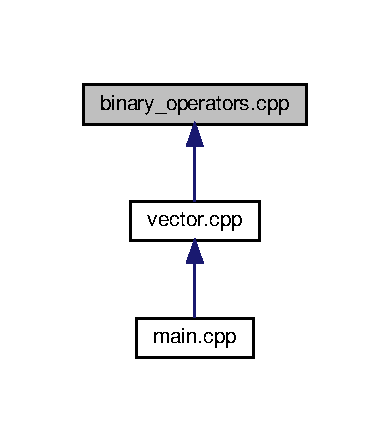
\includegraphics[width=187pt]{binary__operators_8cpp__dep__incl}
\end{center}
\end{figure}
\subsection*{Functions}
\begin{DoxyCompactItemize}
\item 
{\footnotesize template$<$typename data $>$ }\\\hyperlink{classVector}{Vector}$<$ data $>$ \hyperlink{binary__operators_8cpp_a8c8eb33fc89878de6c7a2d869e451482}{operator+} (const \hyperlink{classVector}{Vector}$<$ data $>$ \&v1, const \hyperlink{classVector}{Vector}$<$ data $>$ \&v2)  throw (\+Den\+Exception)
\begin{DoxyCompactList}\small\item\em operator \hyperlink{classVector}{Vector} + \hyperlink{classVector}{Vector} \end{DoxyCompactList}\item 
{\footnotesize template$<$typename data $>$ }\\\hyperlink{classVector}{Vector}$<$ data $>$ \hyperlink{binary__operators_8cpp_a3ca69957de672a02ef4d157935f767f4}{operator-\/} (const \hyperlink{classVector}{Vector}$<$ data $>$ \&v1, const \hyperlink{classVector}{Vector}$<$ data $>$ \&v2)  throw (\+Den\+Exception)
\begin{DoxyCompactList}\small\item\em operator \hyperlink{classVector}{Vector} -\/ \hyperlink{classVector}{Vector} \end{DoxyCompactList}\item 
{\footnotesize template$<$typename data $>$ }\\\hyperlink{classVector}{Vector}$<$ data $>$ \hyperlink{binary__operators_8cpp_a4c9a4f60cd2206296324dfef954befbc}{operator$\ast$} (const \hyperlink{classVector}{Vector}$<$ data $>$ \&v1, double num)  throw (\+Den\+Exception)
\begin{DoxyCompactList}\small\item\em operator \hyperlink{classVector}{Vector} $\ast$ const \end{DoxyCompactList}\item 
{\footnotesize template$<$typename data $>$ }\\\hyperlink{classVector}{Vector}$<$ data $>$ \hyperlink{binary__operators_8cpp_ad4e34c29cad6934dee13b462a132d067}{operator$\ast$} (double num, const \hyperlink{classVector}{Vector}$<$ data $>$ \&v1)  throw (\+Den\+Exception)
\begin{DoxyCompactList}\small\item\em operator const $\ast$ \hyperlink{classVector}{Vector} \end{DoxyCompactList}\item 
{\footnotesize template$<$typename data $>$ }\\\hyperlink{classVector}{Vector}$<$ data $>$ \hyperlink{binary__operators_8cpp_a5650565de6a917334f6c6b149264567d}{operator/} (const \hyperlink{classVector}{Vector}$<$ data $>$ \&v1, double num)  throw (\+Den\+Exception)
\begin{DoxyCompactList}\small\item\em operator \hyperlink{classVector}{Vector} / const \end{DoxyCompactList}\item 
{\footnotesize template$<$typename data $>$ }\\std\+::ostream \& \hyperlink{binary__operators_8cpp_a5e10d56f7663035c54015f1264204212}{operator$<$$<$} (std\+::ostream \&os, const \hyperlink{classVector}{Vector}$<$ data $>$ \&v1)
\begin{DoxyCompactList}\small\item\em output operator  print \hyperlink{classVector}{Vector} to os stream \end{DoxyCompactList}\end{DoxyCompactItemize}


\subsection{Detailed Description}
class description file vector 

\begin{DoxyAuthor}{Author}
Den 
\end{DoxyAuthor}
\begin{DoxyVersion}{Version}
1.\+0 
\end{DoxyVersion}
\begin{DoxyDate}{Date}
March 2019 
\end{DoxyDate}


\subsection{Function Documentation}
\mbox{\Hypertarget{binary__operators_8cpp_a4c9a4f60cd2206296324dfef954befbc}\label{binary__operators_8cpp_a4c9a4f60cd2206296324dfef954befbc}} 
\index{binary\+\_\+operators.\+cpp@{binary\+\_\+operators.\+cpp}!operator$\ast$@{operator$\ast$}}
\index{operator$\ast$@{operator$\ast$}!binary\+\_\+operators.\+cpp@{binary\+\_\+operators.\+cpp}}
\subsubsection{\texorpdfstring{operator$\ast$()}{operator*()}\hspace{0.1cm}{\footnotesize\ttfamily [1/2]}}
{\footnotesize\ttfamily template$<$typename data $>$ \\
\hyperlink{classVector}{Vector}$<$data$>$ operator$\ast$ (\begin{DoxyParamCaption}\item[{const \hyperlink{classVector}{Vector}$<$ data $>$ \&}]{v1,  }\item[{double}]{num }\end{DoxyParamCaption}) throw  Den\+Exception) }



operator \hyperlink{classVector}{Vector} $\ast$ const 


\begin{DoxyParams}[1]{Parameters}
\mbox{\tt in}  & {\em v1} & Vector1 \\
\hline
\mbox{\tt in}  & {\em num} & const \\
\hline
\end{DoxyParams}
\begin{DoxyReturn}{Returns}
result \hyperlink{classVector}{Vector} 
\end{DoxyReturn}

\begin{DoxyExceptions}{Exceptions}
{\em Den\+Exception} & \\
\hline
\end{DoxyExceptions}


Definition at line 66 of file binary\+\_\+operators.\+cpp.


\begin{DoxyCode}
67     \{
68         \hyperlink{classVector}{Vector<data>} copy(v1.\hyperlink{classVector_a81b1d973485244101caf8e901b4a03d9}{size}());
69 
70         \textcolor{keywordflow}{for}(\textcolor{keywordtype}{int} i = 0; i < v1.\hyperlink{classVector_a81b1d973485244101caf8e901b4a03d9}{size}(); i++) copy[i] = v1[i] * num;
71 
72         \textcolor{keywordflow}{return} copy;
73     \}
\end{DoxyCode}
\mbox{\Hypertarget{binary__operators_8cpp_ad4e34c29cad6934dee13b462a132d067}\label{binary__operators_8cpp_ad4e34c29cad6934dee13b462a132d067}} 
\index{binary\+\_\+operators.\+cpp@{binary\+\_\+operators.\+cpp}!operator$\ast$@{operator$\ast$}}
\index{operator$\ast$@{operator$\ast$}!binary\+\_\+operators.\+cpp@{binary\+\_\+operators.\+cpp}}
\subsubsection{\texorpdfstring{operator$\ast$()}{operator*()}\hspace{0.1cm}{\footnotesize\ttfamily [2/2]}}
{\footnotesize\ttfamily template$<$typename data $>$ \\
\hyperlink{classVector}{Vector}$<$data$>$ operator$\ast$ (\begin{DoxyParamCaption}\item[{double}]{num,  }\item[{const \hyperlink{classVector}{Vector}$<$ data $>$ \&}]{v1 }\end{DoxyParamCaption}) throw  Den\+Exception) }



operator const $\ast$ \hyperlink{classVector}{Vector} 


\begin{DoxyParams}[1]{Parameters}
\mbox{\tt in}  & {\em num} & const \\
\hline
\mbox{\tt in}  & {\em v1} & Vector1 \\
\hline
\end{DoxyParams}
\begin{DoxyReturn}{Returns}
result \hyperlink{classVector}{Vector} 
\end{DoxyReturn}

\begin{DoxyExceptions}{Exceptions}
{\em Den\+Exception} & \\
\hline
\end{DoxyExceptions}


Definition at line 86 of file binary\+\_\+operators.\+cpp.


\begin{DoxyCode}
87     \{
88         \textcolor{keywordflow}{return} v1 * num;
89     \}
\end{DoxyCode}
\mbox{\Hypertarget{binary__operators_8cpp_a8c8eb33fc89878de6c7a2d869e451482}\label{binary__operators_8cpp_a8c8eb33fc89878de6c7a2d869e451482}} 
\index{binary\+\_\+operators.\+cpp@{binary\+\_\+operators.\+cpp}!operator+@{operator+}}
\index{operator+@{operator+}!binary\+\_\+operators.\+cpp@{binary\+\_\+operators.\+cpp}}
\subsubsection{\texorpdfstring{operator+()}{operator+()}}
{\footnotesize\ttfamily template$<$typename data $>$ \\
\hyperlink{classVector}{Vector}$<$data$>$ operator+ (\begin{DoxyParamCaption}\item[{const \hyperlink{classVector}{Vector}$<$ data $>$ \&}]{v1,  }\item[{const \hyperlink{classVector}{Vector}$<$ data $>$ \&}]{v2 }\end{DoxyParamCaption}) throw  Den\+Exception) }



operator \hyperlink{classVector}{Vector} + \hyperlink{classVector}{Vector} 


\begin{DoxyParams}[1]{Parameters}
\mbox{\tt in}  & {\em v1} & Vector1 \\
\hline
\mbox{\tt in}  & {\em v2} & Vector2 \\
\hline
\end{DoxyParams}
\begin{DoxyReturn}{Returns}
result \hyperlink{classVector}{Vector} 
\end{DoxyReturn}

\begin{DoxyExceptions}{Exceptions}
{\em Den\+Exception} & \\
\hline
\end{DoxyExceptions}


Definition at line 22 of file binary\+\_\+operators.\+cpp.


\begin{DoxyCode}
23     \{
24         assert(v1.\hyperlink{classVector_a81b1d973485244101caf8e901b4a03d9}{size}() == v2.\hyperlink{classVector_a81b1d973485244101caf8e901b4a03d9}{size}());
25 
26         \hyperlink{classVector}{Vector<data>} copy(v1.\hyperlink{classVector_a81b1d973485244101caf8e901b4a03d9}{size}());
27 
28         \textcolor{keywordflow}{for}(\textcolor{keywordtype}{int} i = 0; i < v1.\hyperlink{classVector_a81b1d973485244101caf8e901b4a03d9}{size}(); i++) copy[i] = v1[i] + v2[i];
29 
30         \textcolor{keywordflow}{return} copy;
31     \}
\end{DoxyCode}
\mbox{\Hypertarget{binary__operators_8cpp_a3ca69957de672a02ef4d157935f767f4}\label{binary__operators_8cpp_a3ca69957de672a02ef4d157935f767f4}} 
\index{binary\+\_\+operators.\+cpp@{binary\+\_\+operators.\+cpp}!operator-\/@{operator-\/}}
\index{operator-\/@{operator-\/}!binary\+\_\+operators.\+cpp@{binary\+\_\+operators.\+cpp}}
\subsubsection{\texorpdfstring{operator-\/()}{operator-()}}
{\footnotesize\ttfamily template$<$typename data $>$ \\
\hyperlink{classVector}{Vector}$<$data$>$ operator-\/ (\begin{DoxyParamCaption}\item[{const \hyperlink{classVector}{Vector}$<$ data $>$ \&}]{v1,  }\item[{const \hyperlink{classVector}{Vector}$<$ data $>$ \&}]{v2 }\end{DoxyParamCaption}) throw  Den\+Exception) }



operator \hyperlink{classVector}{Vector} -\/ \hyperlink{classVector}{Vector} 


\begin{DoxyParams}[1]{Parameters}
\mbox{\tt in}  & {\em v1} & Vector1 \\
\hline
\mbox{\tt in}  & {\em v2} & Vector2 \\
\hline
\end{DoxyParams}
\begin{DoxyReturn}{Returns}
result \hyperlink{classVector}{Vector} 
\end{DoxyReturn}

\begin{DoxyExceptions}{Exceptions}
{\em Den\+Exception} & \\
\hline
\end{DoxyExceptions}


Definition at line 44 of file binary\+\_\+operators.\+cpp.


\begin{DoxyCode}
45     \{
46         assert(v1.\hyperlink{classVector_a81b1d973485244101caf8e901b4a03d9}{size}() == v2.\hyperlink{classVector_a81b1d973485244101caf8e901b4a03d9}{size}());
47 
48         \hyperlink{classVector}{Vector<data>} copy(v1.\hyperlink{classVector_a81b1d973485244101caf8e901b4a03d9}{size}());
49 
50         \textcolor{keywordflow}{for}(\textcolor{keywordtype}{int} i = 0; i < v1.\hyperlink{classVector_a81b1d973485244101caf8e901b4a03d9}{size}(); i++) copy[i] = v1[i] - v2[i];
51 
52         \textcolor{keywordflow}{return} copy;
53     \}
\end{DoxyCode}
\mbox{\Hypertarget{binary__operators_8cpp_a5650565de6a917334f6c6b149264567d}\label{binary__operators_8cpp_a5650565de6a917334f6c6b149264567d}} 
\index{binary\+\_\+operators.\+cpp@{binary\+\_\+operators.\+cpp}!operator/@{operator/}}
\index{operator/@{operator/}!binary\+\_\+operators.\+cpp@{binary\+\_\+operators.\+cpp}}
\subsubsection{\texorpdfstring{operator/()}{operator/()}}
{\footnotesize\ttfamily template$<$typename data $>$ \\
\hyperlink{classVector}{Vector}$<$data$>$ operator/ (\begin{DoxyParamCaption}\item[{const \hyperlink{classVector}{Vector}$<$ data $>$ \&}]{v1,  }\item[{double}]{num }\end{DoxyParamCaption}) throw  Den\+Exception) }



operator \hyperlink{classVector}{Vector} / const 


\begin{DoxyParams}[1]{Parameters}
\mbox{\tt in}  & {\em v1} & Vector1 \\
\hline
\mbox{\tt in}  & {\em num} & const \\
\hline
\end{DoxyParams}
\begin{DoxyReturn}{Returns}
result \hyperlink{classVector}{Vector} 
\end{DoxyReturn}

\begin{DoxyExceptions}{Exceptions}
{\em Den\+Exception} & \\
\hline
\end{DoxyExceptions}


Definition at line 102 of file binary\+\_\+operators.\+cpp.


\begin{DoxyCode}
103     \{
104         \hyperlink{classVector}{Vector<data>} copy(v1.\hyperlink{classVector_a81b1d973485244101caf8e901b4a03d9}{size}());
105 
106         \textcolor{keywordflow}{for}(\textcolor{keywordtype}{int} i = 0; i < v1.\hyperlink{classVector_a81b1d973485244101caf8e901b4a03d9}{size}(); i++) copy[i] = v1[i] / num;
107 
108         \textcolor{keywordflow}{return} copy;
109     \}
\end{DoxyCode}
\mbox{\Hypertarget{binary__operators_8cpp_a5e10d56f7663035c54015f1264204212}\label{binary__operators_8cpp_a5e10d56f7663035c54015f1264204212}} 
\index{binary\+\_\+operators.\+cpp@{binary\+\_\+operators.\+cpp}!operator$<$$<$@{operator$<$$<$}}
\index{operator$<$$<$@{operator$<$$<$}!binary\+\_\+operators.\+cpp@{binary\+\_\+operators.\+cpp}}
\subsubsection{\texorpdfstring{operator$<$$<$()}{operator<<()}}
{\footnotesize\ttfamily template$<$typename data $>$ \\
std\+::ostream\& operator$<$$<$ (\begin{DoxyParamCaption}\item[{std\+::ostream \&}]{os,  }\item[{const \hyperlink{classVector}{Vector}$<$ data $>$ \&}]{v1 }\end{DoxyParamCaption})}



output operator  print \hyperlink{classVector}{Vector} to os stream 


\begin{DoxyParams}[1]{Parameters}
\mbox{\tt in}  & {\em os} & print stream \\
\hline
\mbox{\tt in}  & {\em v1} & \hyperlink{classVector}{Vector} to print \\
\hline
\end{DoxyParams}

\begin{DoxyExceptions}{Exceptions}
{\em Den\+Exception} & \\
\hline
\end{DoxyExceptions}


Definition at line 122 of file binary\+\_\+operators.\+cpp.


\begin{DoxyCode}
123     \{
124         \textcolor{keywordflow}{for}(\textcolor{keywordtype}{int} i = 0; i < v1.\hyperlink{classVector_a81b1d973485244101caf8e901b4a03d9}{size}(); ++i)
125             os << v1[i] << \textcolor{charliteral}{' '};
126         \textcolor{keywordflow}{return} os;
127     \}
\end{DoxyCode}

\hypertarget{bool__vector_8cpp}{}\section{bool\+\_\+vector.\+cpp File Reference}
\label{bool__vector_8cpp}\index{bool\+\_\+vector.\+cpp@{bool\+\_\+vector.\+cpp}}


class bool vector  


This graph shows which files directly or indirectly include this file\+:
\nopagebreak
\begin{figure}[H]
\begin{center}
\leavevmode
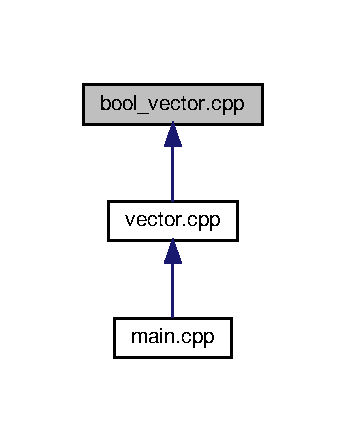
\includegraphics[width=166pt]{bool__vector_8cpp__dep__incl}
\end{center}
\end{figure}
\subsection*{Data Structures}
\begin{DoxyCompactItemize}
\item 
class \hyperlink{classVector_3_01bool_01_4}{Vector$<$ bool $>$}
\begin{DoxyCompactList}\small\item\em Type \hyperlink{classVector_3_01bool_01_4}{Vector$<$bool$>$}. Effective in speed, but spends a lot of memory. \end{DoxyCompactList}\item 
class \hyperlink{classVector_3_01bool_01_4_1_1BoolReference}{Vector$<$ bool $>$\+::\+Bool\+Reference}
\end{DoxyCompactItemize}


\subsection{Detailed Description}
class bool vector 

\begin{DoxyAuthor}{Author}
Den 
\end{DoxyAuthor}
\begin{DoxyVersion}{Version}
1.\+0 
\end{DoxyVersion}
\begin{DoxyDate}{Date}
March 2019 
\end{DoxyDate}

\hypertarget{main_8cpp}{}\section{main.\+cpp File Reference}
\label{main_8cpp}\index{main.\+cpp@{main.\+cpp}}


some example of \hyperlink{classVector}{Vector}  


{\ttfamily \#include \char`\"{}vector.\+cpp\char`\"{}}\newline
Include dependency graph for main.\+cpp\+:
\nopagebreak
\begin{figure}[H]
\begin{center}
\leavevmode
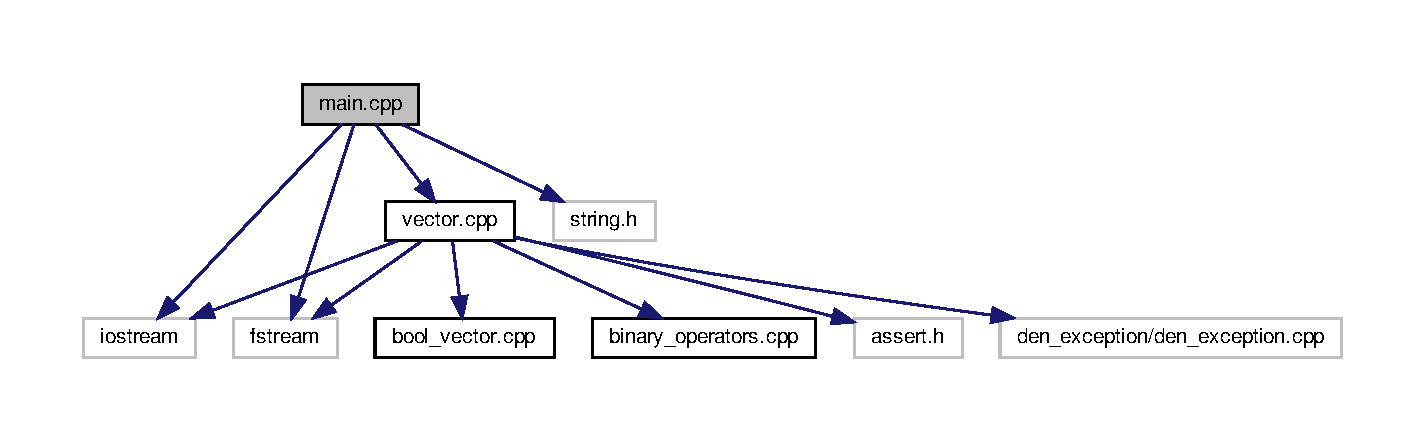
\includegraphics[width=350pt]{main_8cpp__incl}
\end{center}
\end{figure}
\subsection*{Functions}
\begin{DoxyCompactItemize}
\item 
\mbox{\Hypertarget{main_8cpp_a840291bc02cba5474a4cb46a9b9566fe}\label{main_8cpp_a840291bc02cba5474a4cb46a9b9566fe}} 
int {\bfseries main} (void)
\end{DoxyCompactItemize}


\subsection{Detailed Description}
some example of \hyperlink{classVector}{Vector} 

\begin{DoxyAuthor}{Author}
Den 
\end{DoxyAuthor}
\begin{DoxyVersion}{Version}
1.\+0 
\end{DoxyVersion}
\begin{DoxyDate}{Date}
March 2019 
\end{DoxyDate}

\hypertarget{vector_8cpp}{}\section{vector.\+cpp File Reference}
\label{vector_8cpp}\index{vector.\+cpp@{vector.\+cpp}}


class description file vector  


{\ttfamily \#include $<$iostream$>$}\newline
{\ttfamily \#include $<$fstream$>$}\newline
{\ttfamily \#include $<$assert.\+h$>$}\newline
{\ttfamily \#include \char`\"{}den\+\_\+exception/den\+\_\+exception.\+cpp\char`\"{}}\newline
{\ttfamily \#include \char`\"{}bool\+\_\+vector.\+cpp\char`\"{}}\newline
{\ttfamily \#include \char`\"{}binary\+\_\+operators.\+cpp\char`\"{}}\newline
Include dependency graph for vector.\+cpp\+:
\nopagebreak
\begin{figure}[H]
\begin{center}
\leavevmode
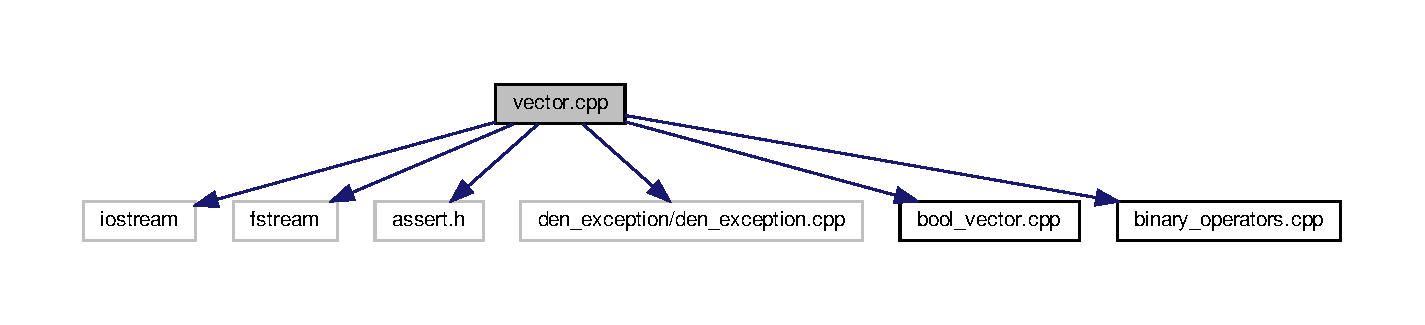
\includegraphics[width=350pt]{vector_8cpp__incl}
\end{center}
\end{figure}
This graph shows which files directly or indirectly include this file\+:
\nopagebreak
\begin{figure}[H]
\begin{center}
\leavevmode
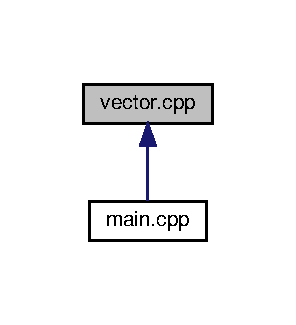
\includegraphics[width=142pt]{vector_8cpp__dep__incl}
\end{center}
\end{figure}
\subsection*{Data Structures}
\begin{DoxyCompactItemize}
\item 
class \hyperlink{classVector}{Vector$<$ data $>$}
\begin{DoxyCompactList}\small\item\em Type \hyperlink{classVector}{Vector}. Effective in speed, but spends a lot of memory. \end{DoxyCompactList}\end{DoxyCompactItemize}
\subsection*{Macros}
\begin{DoxyCompactItemize}
\item 
\mbox{\Hypertarget{vector_8cpp_a0e56521e7ab51dee5a9705e070406265}\label{vector_8cpp_a0e56521e7ab51dee5a9705e070406265}} 
\#define {\bfseries V\+E\+C\+T\+O\+R\+\_\+H}
\item 
\mbox{\Hypertarget{vector_8cpp_a0881bd0885196a40e66cc0f9ff435723}\label{vector_8cpp_a0881bd0885196a40e66cc0f9ff435723}} 
\#define {\bfseries D\+E\+N\+\_\+\+E\+X\+C\+E\+P\+T\+I\+ON}(message,  exc\+\_\+code)~Den\+Exception(\+\_\+\+\_\+\+F\+I\+L\+E\+\_\+\+\_\+, \+\_\+\+\_\+func\+\_\+\+\_\+, \+\_\+\+\_\+\+L\+I\+N\+E\+\_\+\+\_\+, message, exc\+\_\+code)
\item 
\mbox{\Hypertarget{vector_8cpp_ab6bca16ed021b1e211fde8669758f199}\label{vector_8cpp_ab6bca16ed021b1e211fde8669758f199}} 
\#define {\bfseries N\+EW}~new(\+\_\+\+\_\+\+F\+I\+L\+E\+\_\+\+\_\+, \+\_\+\+\_\+func\+\_\+\+\_\+, \+\_\+\+\_\+\+L\+I\+N\+E\+\_\+\+\_\+, memory\+\_\+leak)
\item 
\#define {\bfseries D\+E\+L\+E\+TE}(x)
\end{DoxyCompactItemize}
\subsection*{Functions}
\begin{DoxyCompactItemize}
\item 
\mbox{\Hypertarget{vector_8cpp_aba3799ff09b5cbeeb120156b2c804ca8}\label{vector_8cpp_aba3799ff09b5cbeeb120156b2c804ca8}} 
std\+::ofstream {\bfseries memory\+\_\+leak} (\char`\"{}memory\+\_\+leak/memory\+\_\+leak.\+txt\char`\"{})
\end{DoxyCompactItemize}


\subsection{Detailed Description}
class description file vector 

\begin{DoxyAuthor}{Author}
Den 
\end{DoxyAuthor}
\begin{DoxyVersion}{Version}
1.\+0 
\end{DoxyVersion}
\begin{DoxyDate}{Date}
March 2019 
\end{DoxyDate}


\subsection{Macro Definition Documentation}
\mbox{\Hypertarget{vector_8cpp_a9f91c27f0bcb26ae76eb4d51e5a0aca5}\label{vector_8cpp_a9f91c27f0bcb26ae76eb4d51e5a0aca5}} 
\index{vector.\+cpp@{vector.\+cpp}!D\+E\+L\+E\+TE@{D\+E\+L\+E\+TE}}
\index{D\+E\+L\+E\+TE@{D\+E\+L\+E\+TE}!vector.\+cpp@{vector.\+cpp}}
\subsubsection{\texorpdfstring{D\+E\+L\+E\+TE}{DELETE}}
{\footnotesize\ttfamily \#define D\+E\+L\+E\+TE(\begin{DoxyParamCaption}\item[{}]{x }\end{DoxyParamCaption})}

{\bfseries Value\+:}
\begin{DoxyCode}
memory\_leak << \textcolor{stringliteral}{"D "} << \_\_FILE\_\_ << \textcolor{stringliteral}{"|"} << \_\_func\_\_ << \textcolor{stringliteral}{"|"} << \_\_LINE\_\_ << \textcolor{stringliteral}{" "} << x << std::endl; \(\backslash\)
                delete x;
\end{DoxyCode}


Definition at line 504 of file vector.\+cpp.


%--- End generated contents ---

% Index
\backmatter
\newpage
\phantomsection
\clearemptydoublepage
\addcontentsline{toc}{chapter}{Index}
\printindex

\end{document}
